%
% File acl2017.tex
%
%% Based on the style files for ACL-2015, with some improvements
%%  taken from the NAACL-2016 style
%% Based on the style files for ACL-2014, which were, in turn,
%% based on ACL-2013, ACL-2012, ACL-2011, ACL-2010, ACL-IJCNLP-2009,
%% EACL-2009, IJCNLP-2008...
%% Based on the style files for EACL 2006 by 
%%e.agirre@ehu.es or Sergi.Balari@uab.es
%% and that of ACL 08 by Joakim Nivre and Noah Smith

\documentclass[11pt,a4paper]{article}
\usepackage[hyperref]{acl2017}
\usepackage{times}
\usepackage{latexsym}

\usepackage{url}

\aclfinalcopy % Uncomment this line for the final submission
\def\aclpaperid{684} %  Enter the acl Paper ID here

%\setlength\titlebox{5cm}
% You can expand the titlebox if you need extra space
% to show all the authors. Please do not make the titlebox
% smaller than 5cm (the original size); we will check this
% in the camera-ready version and ask you to change it back.

\newcommand\BibTeX{B{\sc ib}\TeX}

\usepackage{url}
\usepackage{times}
\usepackage{latexsym}
\usepackage{graphicx}
\usepackage{booktabs}
\usepackage{amsmath}
\usepackage{amssymb}
%\usepackage[colorlinks=true]{hyperref}
\usepackage{booktabs}
\usepackage{multirow}
\newcommand{\red}[1]{\textcolor{red}{#1}}
\newcommand{\blue}[1]{\textcolor{blue}{#1}}
\usepackage{caption}
\usepackage{subcaption}
\usepackage{soul}
\usepackage{float}
\usepackage{wrapfig}
\DeclareMathOperator{\bigru}{\overset{\longleftrightarrow}{\mathrm{GRU}}}
% \setlength{\textfloatsep}{2em} 
\captionsetup[table]{aboveskip=6pt}
\usepackage{xcolor}
\definecolor{darkblue}{rgb}{0.0, 0.0, 0.55}
\hypersetup{citecolor=darkblue}

\title{Gated-Attention Readers for Text Comprehension}

\author{Bhuwan Dhingra\thanks{\enskip BD and HL contributed equally to this work.}\qquad Hanxiao Liu\footnotemark[1]\qquad Zhilin Yang\\ {\bf William W. Cohen \qquad Ruslan Salakhutdinov} \\
School of Computer Science\\
Carnegie Mellon University\\
\texttt{\{bdhingra,hanxiaol,zhiliny,wcohen,rsalakhu\}@cs.cmu.edu}}
\date{}

\begin{document}

\maketitle

\begin{abstract}
In this paper we study the problem of answering cloze-style questions over documents. Our model, the Gated-Attention (GA) Reader\footnote{Source code is available on github: \url{https://github.com/bdhingra/ga-reader}}, integrates a multi-hop architecture with a novel attention mechanism, which is based on multiplicative interactions between the query embedding and the intermediate states of a recurrent neural network document reader. This enables the reader to build query-specific representations of tokens in the document for accurate answer selection. The GA Reader obtains state-of-the-art results on three benchmarks for this task--the CNN \& Daily Mail news stories and the Who Did What dataset.
The effectiveness of multiplicative interaction is demonstrated by an ablation study,
and by comparing to alternative compositional operators for implementing the gated-attention. 
% We further demonstrate the effectiveness of multiplicative attention for this task by performing an ablation study without it, and by comparing to other types of gating operations between the query and document.
% We also provide a detailed analysis of the performance of our model and several baselines over a subset of questions manually annotated with certain linguistic features. The analysis sheds light on the strengths and weaknesses of several existing models.
\end{abstract}

\section{Introduction}
A recent trend to measure progress towards machine reading is to test a system's ability to answer questions about a document it has to comprehend. Towards this end, several large-scale datasets of cloze-style questions over a context document have been introduced recently, which allow the training of supervised machine learning systems \citep{hermann2015teaching,hill2015goldilocks,onishi2016did}. Such datasets can be easily constructed automatically and the unambiguous nature of their queries provides an objective benchmark to measure a system's performance at text comprehension. 

% \hl{todo: update the remaining parts of intro sec}

% Deep learning methods have recently been shown to outperform traditional shallow approaches on reading comprehension tasks \citep{hermann2015teaching}. Their performance is further boosted by attention mechanisms borrowed from the machine translation literature \citep{bahdanau2014neural}. This is not surprising, 
% %since anyone who has attempted to answer a cloze-style query will testify that the best approach 
% as answering a cloze-style query requires one 
% to only attend to parts of the document relevant to the query. Current attention models aim to mimic this by weighting representations of document sub-units (such as words or sentences) by a score which determines their relevance to the query \citep{hermann2015teaching,hill2015goldilocks,kadlec2016text}. 

% An alternative way to selectively ``attend'' to different parts of the document while reading it is by gating the input to the reader with the query representation. This can be intuitively viewed as masking unimportant features of the input (for the task at hand) and emphasizing the important ones. Specifically, we compute an element-wise product between the query embedding  and document representations at the intermediate layers of a Bidirectional Gated Recurrent Unit (GRU) \citep{cho2014learning} reader. Our method was inspired by the observation that the GRU itself provides an attention mechanism through the use of its reset and forget gates; the element-wise product simply helps it focus on the query. We call this model the Gated-Attention (GA) Reader. The effectiveness of the proposed gated-attention mechanism is verified by the consistent improvement of the GA reader over various existing models on three different benchmark datasets.

% The paper is organized as follows:
% We discuss related models in Section \ref{sec:related}
% and then introduce the GA Reader in Section \ref{sec:ga}.
% Experiment results are presented in Section \ref{sec:results}.
% We summarize our findings in Section \ref{sec:conclusion}.
Deep learning models have been shown to outperform traditional shallow approaches
on text comprehension tasks \citep{hermann2015teaching}.
The success of many recent models can be attributed primarily to two factors:
(1) \emph{Multi-hop architectures} 
\citep{weston2014memory, sordoni2016iterative, shen2016reasonet},
allow a model to scan the document and the question iteratively for multiple passes.
(2) \emph{Attention mechanisms},
\citep{chen2016thorough, hermann2015teaching}
borrowed from the machine translation literature \citep{bahdanau2014neural},
allow the model to focus on appropriate subparts of the context document.
Intuitively,
the multi-hop architecture allows the reader to incrementally refine token representations,
and the attention mechanism re-weights different parts in the document according to their relevance to the query.

The effectiveness of multi-hop reasoning and attentions have been explored orthogonally so far
in the literature.
In this paper,
we focus on combining both in a complementary manner,
by designing a novel attention mechanism which gates the evolving token representations across hops.
More specifically,
unlike existing models where the query attention
is applied either token-wise \citep{hermann2015teaching, kadlec2016text, chen2016thorough, hill2015goldilocks} or
sentence-wise \citep{weston2014memory, sukhbaatar2015end} to allow weighted aggregation,
the Gated-Attention (GA) module proposed in this work allows the query to directly interact with each dimension
of the token embeddings at the semantic-level,
and is applied layer-wise as information filters during the multi-hop representation learning process.
Such a fine-grained attention enables our model to learn conditional token representations w.r.t.\ the given question,
leading to accurate answer selections. 

We show in our experiments that the proposed GA reader,
despite its relative simplicity,
consistently improves over a variety of strong baselines on three benchmark datasets
. 
Our key contribution, the GA module, provides a significant improvement for large datasets. Qualitatively, visualization of the attentions at intermediate layers of the GA reader shows that in each layer the GA reader attends to distinct salient aspects of the query which help in determining the answer. 

\section{Related Work}
\label{sec:related}
The cloze-style QA task involves tuples of the form $(d,q,a,\mathcal{C})$, where $d$ is a document (context), $q$ is a query over the contents of $d$, in which a phrase is replaced with a placeholder, and $a$ is the answer to $q$, which comes from a set of candidates $\mathcal{C}$. In this work we consider datasets where each candidate $c \in \mathcal{C}$ has at least one token which also appears in the document. The task can then be described as: given a document-query pair $(d,q)$, find $a \in \mathcal{C}$ which answers $q$. Below we provide an overview of representative neural network architectures which have been applied to this problem.

\textit{LSTMs with Attention:} Several architectures introduced in \citet{hermann2015teaching}
employ LSTM units to compute a combined document-query representation $g(d,q)$,
which is used to rank the candidate answers.
These include the \textbf{DeepLSTM Reader} which performs a single forward pass through the concatenated \textit{(document, query)} pair to obtain $g(d,q)$;
the \textbf{Attentive Reader} which first computes a document vector $d(q)$ by a weighted aggregation of words according to attentions based on $q$, and then combines $d(q)$ and $q$ to obtain their joint representation $g(d(q),q)$;
and the \textbf{Impatient Reader} where the document representation is built incrementally.
The architecture of the Attentive Reader has been simplified recently in \textbf{Stanford Attentive Reader},
where shallower recurrent units were used with a bilinear form for the query-document attention \citep{chen2016thorough}.

\textit{Attention Sum:} The \textbf{Attention-Sum (AS) Reader}
\citep{kadlec2016text} uses two bi-directional GRU networks \citep{cho2014learning} to encode both $d$ and $q$ into vectors.
A probability distribution over the entities in $d$
is obtained by computing dot products between $q$ and the entity embeddings and taking a softmax. 
Then, an aggregation scheme named \emph{pointer-sum attention}
is further applied to sum the probabilities of the same entity,
so that frequent entities the document will be favored
compared to rare ones. 
Building on the AS Reader,
the \textbf{Attention-over-Attention (AoA) Reader} \citep{cui2016attention} 
introduces a two-way attention mechanism where the query and the document are mutually attentive to each other.

\textit{Mulit-hop Architectures:} \textbf{Memory Networks (MemNets}) were proposed in \citet{weston2014memory},
%and have been applied to the Children's Book Test \citep{hill2015goldilocks}.
where each sentence in the document is encoded to a memory by aggregating nearby words. 
Attention over the memory slots given the query is used to compute an overall memory and to renew the query representation over multiple iterations, allowing certain types of reasoning over the salient facts in the memory and the query. 
%In each iteration, the model can select a relevant memory and add it to the input for the next hop.
\textbf{Neural Semantic Encoders (NSE)} \citep{munkhdalai2016neural} extended MemNets by introducing a \textit{write} operation which can evolve the memory over time during the course of reading.
Iterative reasoning has been found effective in several more recent models,
including the \textbf{Iterative Attentive Reader} \citep{sordoni2016iterative} and \textbf{ReasoNet} \citep{shen2016reasonet}.
The latter allows dynamic reasoning steps
and is trained with reinforcement learning. 

% Then, candidate answers which appear in the document are evaluated by extracting their contextual representations from the bi-GRU and taking a dot-product with the query vector $q$. This gives a score for each possible answer, which is normalized by the softmax function. Finally, multiple mentions of the same candidate entity are combined by adding up their probabilities, and the token with the maximum aggregated probability is selected as the predicted answer. This aggregation scheme is known as the \textit{pointer sum attention}.

Other related works include \textbf{Dynamic Entity Representation network (DER}) \citep{kobayashi2016dynamic},
which builds dynamic representations of the candidate answers while reading the document, and accumulates the information about an entity by max-pooling;
\textbf{EpiReader} \citep{trischler2016natural}
consists of two networks, where one proposes a small set of candidate answers, and the other reranks the proposed candidates conditioned on the query and the context; \textbf{Bi-Directional Attention Flow network (BiDAF)} \cite{seo2016bidirectional} adopts a multi-stage hierarchical architecture along with a flow-based attention mechanism;
\citet{bajgar2016embracing} showed a 10\% improvement on the CBT corpus \citep{hill2015goldilocks} by training the AS Reader on an augmented training set of about 14 million examples, making a case for the community to exploit data abundance. The focus of this paper, however, is on designing models which exploit the available data efficiently.

\section{Gated-Attention Reader}
\label{sec:ga}
% Our method extends the Attention Sum (AS) Reader, and performs multiple hops over the input document similar to the Memory Networks architecture \citep{sukhbaatar2015end}. We use the same \textit{pointer sum attention} mechanism as the AS reader in the output layer to obtain a distribution over candidate answers. End-to-end memory networks have been shown to perform well on synthetic QA tasks which require reasoning over multiple input sentences, and a key reason for this is its multi-layered architecture which performs several passes over the context \citep{sukhbaatar2015end}. Based on these findings we also incorporate multiple layers in our model.

% Our key contribution, however, is in a \textit{gated-attention mechanism}, where after the first layer, subsequent hops over the document are gated by the query representation using an element-wise combination at layer \textit{inputs} (Figure \ref{fig:model}). This is in contrast to conventional attention mechanisms which apply a weighted averaging of layer \textit{outputs} with the weights determined by a dot-product between query and document, e.g., attention mechanisms in all architectures discussed in section \ref{sec:related}. 

% Compositional operators for merging vector space representations of text have been studied extensively in the literature without a clear consensus on the best one. Depending on the task at hand, in some cases addition seems to perform better (for example when composing phrase representations \citep{mitchell2008vector}), in others multiplication does better (for example when modeling entity relations \citep{yang2014learning}). In our experiments, we explored both addition and multiplication as well as concatenation for the element-wise gating operation discussed above, and multiplication performed best. Previously, \citep{kiros2014multiplicative} also used multiplicative interactions between text attributes (such as author information) and word embeddings to derive context-dependent text representations. For the GA reader, the query representation can also be viewed as an attribute conditioned on which we want to learn the relevant document representation. 
Our proposed GA readers perform multiple hops over the document (context), similar to the Memory Networks architecture \citep{sukhbaatar2015end}.
Multi-hop architectures mimic the multi-step comprehension process of human readers,
and have shown promising results in several recent models for text comprehension \citep{sordoni2016iterative, kumar2015ask, shen2016reasonet}.
The contextual representations in GA readers,
namely the embeddings of words in the document,
are iteratively refined across hops
until reaching a final attention-sum module \citep{kadlec2016text} which maps 
the contextual representations in the last hop to a probability distribution over candidate answers.

% why introduce attention
The attention mechanism has been introduced recently to model human focus,
leading to significant improvement in machine translation and image captioning \citep{bahdanau2014neural, mnih2014recurrent}.
In reading comprehension tasks, ideally,
the semantic meanings carried by the contextual embeddings should be aware of the query across hops.
As an example,
human readers are able to keep the question in mind during multiple passes of reading,
to successively mask away information irrelevant to the query.
However,
existing neural network readers are restricted to either attend to tokens \citep{hermann2015teaching, chen2016thorough}
or entire sentences \citep{weston2014memory}, with the assumption that certain sub-parts of the document are more important than others.
In contrast, 
we propose a finer-grained model which attends to components of the semantic representation being built up by the GRU.
The new attention mechanism,
called \emph{gated-attention},
is implemented via \emph{multiplicative} interactions between the query and the contextual embeddings,
and is applied per hop to act as fine-grained information filters during the multi-step reasoning. The filters weigh individual components of the vector representation of \textit{each} token in the document separately.

The design of gated-attention layers is motivated by the effectiveness of multiplicative interaction
among vector-space representations,
e.g., in various types of recurrent units \citep{hochreiter1997long, wu2016multiplicative} and in relational learning \citep{yang2014learning, kiros2014multiplicative}.
While other types of compositional operators are possible,
such as concatenation or addition \citep{mitchell2008vector},
we find that multiplication has strong empirical performance
(section \ref{sec:ablation}),
where query representations naturally serve as information filters
across hops.
% Intuitively,
% multiplicative interaction $e \odot q$ between the entity embedding $e$ and $q$adjusts the semantic meaning of $e$ towards $q$.

\subsection{Model Details}
\label{sec:model-details}
Several components of the model use a Gated Recurrent Unit (GRU) \citep{cho2014learning} which maps an input sequence $X = [x_1,x_2,\ldots,x_T]$ to an ouput sequence $H=[h_1,h_2,\ldots,h_T]$ as follows:
\begin{align*}
r_t &= \sigma (W_r x_t + U_r h_{t-1} + b_r), \\
z_t &= \sigma (W_z x_t + U_z h_{t-1} + b_z), \\
\tilde{h}_t &= \tanh(W_h x_t + U_h (r_t \odot h_{t-1}) + b_h), \\
h_t &= (1-z_t) \odot h_{t-1} + z_t \odot \tilde{h}_t.
\end{align*}
where $\odot$ denotes the Hadamard product or the element-wise multiplication.
$r_t$ and $z_t$ are called the \textit{reset} and \textit{update} gates respectively, and $\tilde{h}_t$ the \textit{candidate output}. 
A Bi-directional GRU (Bi-GRU) processes the sequence in both forward and backward directions to produce two sequences $[h_1^f, h_2^f, \dots, h_T^f ]$ and $[ h_1^b, h_2^b, \dots, h_T^b ]$, which are concatenated at the output
\begin{equation}
    \bigru(X) = [h^f_1 \Vert h^b_T,\ldots,h^f_T \Vert h^b_1]
\end{equation}
where $\bigru(X)$ denotes the \textit{full output} of the Bi-GRU obtained by concatenating each forward state $h^f_i$ and backward state $h^b_{T-i+1}$ at step $i$ given the input $X$. Note $\bigru(X)$ is a matrix in $\mathbb{R}^{2n_h \times T}$ where $n_h$ is the number of hidden units in GRU.

Let $X^{(0)} = [x_1^{(0)},x_2^{(0)},\ldots x_{|D|}^{(0)}]$ denote the token embeddings of the document, which are also inputs at layer 1 for the document reader below, and $Y = [y_1,y_2,\ldots y_{|Q|}]$ denote the token embeddings of the query. Here $|D|$ and $|Q|$ denote the document and query lengths respectively.

%We define the following three combination operations for these two sequences which, together with the equations above, define functions over the input $X$:
%\setlength{\leftmargini}{2.0em}
%\begin{itemize}
%\item[--] $\Psi(X) = H^f \oplus H^b = [h^f_1 \Vert h^b_T,\ldots,h^f_T \Vert h^b_1]$
%\item[--] $\phi(X) = h^f_T \Vert h^b_T$ denotes the \textit{final output} of the Bi-GRU obtained by concatenating final forward and backward states.
%\item[--] $\theta(X,i) = \Psi(X)_i = h^f_i \Vert h^b_{T-i+1}$ denotes the \textit{intermediate output} of the Bi-GRU obtained by concatenating the forward and backward states for input at time-step $i$. 
%\end{itemize} 
%Note that if $d$ is the number of hidden units in each GRU, $\Psi(X)$ is a matrix of size $2d \times T$ and $\phi(X)$ and $\theta(X,i)$ are size $2d$ vectors.

\begin{figure*}[t]
\centering
\caption{Gated-Attention Reader. Dashed lines represent dropout connections.}
%\hspace{0.5cm}
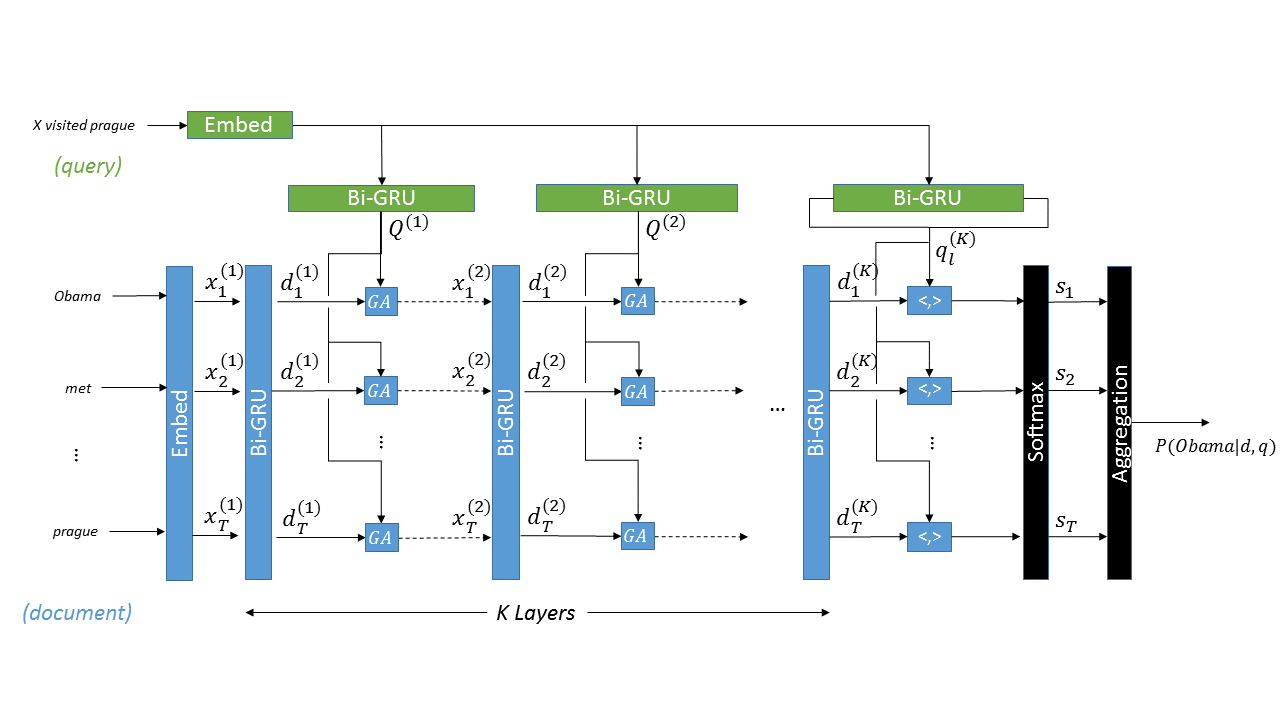
\includegraphics[width=\linewidth,trim={0 25mm 0 25mm},clip]{ga_reader.png}
\label{fig:model}
\end{figure*}

\subsubsection{Multi-Hop Architecture}
Fig.\ \ref{fig:model} illustrates the Gated-Attention (GA) reader. 
The model reads the document and the query over $K$ horizontal layers,
where layer $k$ receives the contextual embeddings $X^{(k-1)}$ of the document from the previous layer. The document embeddings are transformed by taking the full output of a document Bi-GRU (indicated in blue in Fig.\ \ref{fig:model}):
\begin{equation}
    D^{(k)} = \bigru^{(k)}_D(X^{(k-1)})
\end{equation}
At the same time, a layer-specific query representation is computed as the full output of a separate query Bi-GRU (indicated in green in Figure \ref{fig:model}):
\begin{equation}
    Q^{(k)} = \bigru^{(k)}_Q(Y)
\end{equation}

Next, \textit{Gated-Attention} is applied to $D^{(k)}$ and $Q^{(k)}$ to compute inputs for the next layer $X^{(k)}$.
\begin{equation}
    X^{(k)} = \mathrm{GA}(D^{(k)}, Q^{(k)})
\end{equation}
where GA is defined in the following subsection.

\subsubsection{Gated-Attention Module}
For brevity,
let us drop the superscript $k$ in this subsection as we are focusing on a particular layer.
For each token $d_i$ in $D$,
the GA module forms a token-specific representation of the query $\tilde{q}_i$ using soft attention, and then multiplies the query representation element-wise with the document token representation. Specifically, for $i=1,\ldots,|D|$:
\begin{align}
    \alpha_i &= \text{softmax}(Q^\top d_i) \label{eq:q_att} \\
\tilde{q}_i &= Q\alpha_i \nonumber \\
x_i &= d_i \odot \tilde{q}_i
\label{eq:gating}
\end{align}
In equation \eqref{eq:gating} we use the multiplication operator
to model the interactions between $d_i$ and $\tilde{q}_i$.
In the experiments section,
we also report results for other choices of gating functions,
including addition $x_i = d_i + \tilde{q}_i$ and concatenation $x_i = d_i \Vert \tilde{q}_i$.

% At each layer, we combine the final forward and backward GRU hidden states to get the layer-specific query vector:
% \begin{equation}
% q^i = h^f_{|Q|}(i) || h^b_0(i), \qquad i = 1,2,...K,
% \end{equation}
% where $||$ stands for concatenation, $|Q|$ is the query length, and $h^f_t(i)$ and $h^b_t(i)$ are forward and backward GRU hidden states at time $t$ in layer $i$, respectively. GRUs which encode the query are shown in green in the figure. 

% For the document, input at the first Bi-GRU layer consists of word embeddings for the words in the document $x^1_t = L(w_t)$, where $L \in \mathrm{R}^{|V| \times d_L}$ is the word-lookup table, and $w_t$ are indices into the word vocabulary. To compute the input to subsequent Bi-GRU layers, we use the \textit{Gated-Attention} mechanism by applying an element-wise multiplication between the query embedding $q^{i-1}$ and the outputs $e^{i-1}_t$ from the previous layer:
% \begin{equation}
% x^i_t = q^{i-1} \odot e^{i-1}_t, \quad t = 1,2,...|d|. \quad i = 2,...K.
% \end{equation}
% Here $|d|$ is the document length and $\odot$ represents element-wise multiplication (a.k.a. Hadamard product). Layer outputs $e^i_t$ are the contextual embeddings of document tokens formed by concatenating intermediate forward and backward GRU hidden states:
% \begin{equation}
% e^i_t = h^f_t(i) || h^b_t(i), \quad t = 1,2,...|d|. \quad i = 1,...K.
% \end{equation}

\subsubsection{Answer Prediction}
%Let $q^{(K)}_p = \theta^{(K)}_Q(Q,p)$
Let $q^{(K)}_\ell = q_\ell^f\Vert q^b_{T-\ell+1}$ be an intermediate output of the final layer query Bi-GRU at the location $\ell$ of the cloze token in the query,
and $D^{(K)} = \bigru^{(K)}_D(X^{(K-1)})$ be the full output of final layer document Bi-GRU. To obtain the probability that a particular token in the document answers the query, we take an inner-product between these two, and pass through a softmax layer:
\begin{equation}
\label{eq:att}
s = \text{softmax}((q^{(K)}_\ell)^T D^{(K)})
\end{equation}
% \begin{equation}
% \label{eq:att}
% s_t = \frac{\exp \{\langle q^K,e^K_t \rangle \}}{\sum_{t'} \exp\{\langle q^K,e^K_{t'} \rangle \}}, \quad t = 1,2,...|d|,
% \end{equation}
% where $\langle,\rangle$ denotes dot-product between two vectors. 
where vector $s$ defines a probability distribution over the $|D|$ tokens in the document. The probability of a particular candidate $c \in \mathcal{C}$ as being the answer is then computed by aggregating the probabilities of all document tokens which appear in $c$ and renormalizing over the candidates:
\begin{equation}
    \Pr(c|d,q) \propto \sum_{i\in \mathbb{I}(c,d)} s_i
\end{equation}
where $\mathbb{I}(c,d)$ is the set of positions where a token in $c$ appears in the document $d$. This aggregation operation is the same as the \textit{pointer sum attention} applied in the AS Reader \citep{kadlec2016text}.

Finally, the candidate with maximum probability is selected as the predicted answer:
\begin{equation}
    a^* = \mathrm{argmax}_{c \in \mathcal{C}} \enskip \Pr(c|d,q).
\end{equation}

During the training phase,
model parameters of GA are updated w.r.t.\ a cross-entropy loss between the predicted probabilities and the true answers.
%In the special case where $K=1$, the above GA reader reduces to the Attention-Sum Reader.

\subsubsection{Further Enhancements}
\label{sec:tricks}
\emph{Character-level Embeddings}: Given a token $w$ from the document or query, its vector space representation is computed as $x=L(w) || C(w)$. $L(w)$ retrieves the word-embedding for $w$ from a lookup table $L \in \mathbb{R}^{|V|\times n_l}$, whose rows hold a vector for each unique token in the vocabulary. We also utilize a character composition model $C(w)$ which generates an orthographic embedding of the token. Such embeddings have been previously shown to be helpful for tasks like Named Entity Recognition \citep{yang2016multi} and dealing with OOV tokens at test time \citep{dhingra2016tweet2vec}. The embedding $C(w)$ is generated by taking the final outputs $z^f_{n_c}$ and $z^b_{n_c}$ of a Bi-GRU applied to embeddings from a lookup table of characters in the token, and applying a linear transformation:
\begin{align*}
z &= z^f_{n_c} || z^b_{n_c}\\
C(w) &= W z + b
\end{align*}

\emph{Question Evidence Common Word Feature (qe-comm)}: \citet{li2016dataset} recently proposed a simple token level indicator feature which significantly boosts reading comprehension performance in some cases. For each token in the document we construct a one-hot vector $f_i \in \{0,1\}^2$ indicating its presence in the query. It can be incorporated into the GA reader by assigning a feature lookup table $F \in \mathbb{R}^{n_F \times 2}$ (we use $n_F=2$), taking the feature embedding $e_i=f_i^T F$ and appending it to the inputs of the last layer document BiGRU as, $x_i^{(K)} \Vert f_i$ for all $i$. We conducted several experiments both with and without this feature and observed some interesting trends, which are discussed below. Henceforth, we refer to this feature as the \textit{qe-comm feature} or just \textit{feature}.

\section{Experiments and Results}
\label{sec:results}
% \vspace{-0.05in}
\subsection{Datasets}
% \begin{table}[t]
% \small
% \centering
% \caption{Dataset statistics.}
% \label{tab:data}
% \begin{tabular}{@{}ccccl@{}}
% \toprule
% \textbf{Dataset} & \textbf{\#Train} & \textbf{\#Val} & \textbf{\#Test} & \textbf{\#Vocab} \\ \midrule
% CNN              & 380,298             & 3,924               & 3,198              & 118,497             \\
% Daily Mail        & 879,450             & 64,835              & 53,182             & 208,045             \\
% CBT-NE           & 108,719             & 2,000               & 2,500              & 53,063              \\
% CBT-CN           & 120,769             & 2,000               & 2,500              & 53,185              \\ \bottomrule
% \end{tabular}
% \end{table}

We evaluate the GA reader on five large-scale datasets recently proposed in the literature. The first two, CNN and Daily Mail news stories\footnote{\scriptsize \url{https://github.com/deepmind/rc-data}} consist of articles from the popular CNN and Daily Mail websites \citep{hermann2015teaching}. A query over each article is formed by removing an entity from the short summary which follows the article. Further, entities within each article were anonymized to make the task purely a comprehension one. N-gram statistics, for instance, computed over the entire corpus are no longer useful in such an anonymized corpus.

The next two datasets are formed from two different subsets of the Children's Book Test (CBT)\footnote{\scriptsize \url{http://www.thespermwhale.com/jaseweston/babi/CBTest.tgz}} \citep{hill2015goldilocks}. Documents consist of 20 contiguous sentences from the body of a popular children's book, and queries are formed by deleting a token from the 21\textsuperscript{st} sentence. We only focus on subsets where the deleted token is either a common noun (CN) or named entity (NE) since simple language models already give human-level performance on the other types (cf. \citep{hill2015goldilocks}).

The final dataset is Who Did What\footnote{\scriptsize \url{ https://tticnlp.github.io/who_did_what/}} (WDW) \citep{onishi2016did},
constructed from the LDC English Gigaword newswire corpus.
First, article pairs which appeared around the same time and with overlapping entities are chosen, and then one article forms the document and a cloze query is constructed from the other. Missing tokens are always person named entities.
Questions which are easily answered by simple baselines are filtered out,
to make the task more challenging. There are two versions of the training set---a small but focused ``Strict'' version and a large but noisy ``Relaxed'' version.
We report results on both settings which share the same validation and test sets. Statistics of all the datasets used in our experiments are summarized in the Appendix (Table~\ref{tab:data}).

\subsection{Performance Comparison}

\begin{table*}[ht]
\parbox{.60\linewidth}{
\centering
\caption{\small Validation/Test accuracy (\%) on WDW dataset for both ``Strict'' and ``Relaxed'' settings. Results with ``$\dagger$'' are cf previously published works.}
\label{tab:wdw}
\begin{tabular}{l|cc|cc}
\toprule
\multirow{2}{*}{\textbf{Model}}  & \multicolumn{2}{c|}{\textbf{Strict}}              & \multicolumn{2}{c}{\textbf{Relaxed}}              \\ \cmidrule(l){2-5} 
                        & \multicolumn{1}{c|}{Val} & Test          & \multicolumn{1}{c|}{Val} & Test          \\ \midrule
Human  $\dagger$                 & --                       & 84          & --                       & --            \\ \midrule
Attentive Reader   $\dagger$     & --                       & 53          & --                       & 55         \\
AS Reader   $\dagger$            & --                       & 57          & --                       & 59          \\
Stanford AR    $\dagger$         & --                       & 64          & --                       & 65          \\
NSE $\dagger$& 66.5                     & 66.2          & 67.0                     & 66.7          \\ \midrule
GA-{}-  $\dagger$             & --                     & 57          & --                     & 60.0          \\
GA (update $L(w)$)              & 67.8                     & 67.0          & 67.0                     & 66.6          \\
GA (fix $L(w)$)              & 68.3                     & 68.0          & 69.6                     & 69.1          \\
GA (+feature, update $L(w)$)    & 70.1            & 69.5 & 70.9            & 71.0 \\
GA (+feature, fix $L(w)$)    & \textbf{71.6}            & \textbf{71.2} & \textbf{72.6}            & \textbf{72.6} \\\bottomrule
\end{tabular}
}
\hfill
\parbox{.375\linewidth}{
\centering
\caption{\small \textbf{Top:} Performance of different gating functions. \textbf{Bottom:} Effect of varying the number of hops $K$. Results on WDW without using the qe-comm feature and with fixed $L(w)$.}
\label{tab:gating_fn}
\begin{tabular}{@{}l|c|c@{}}
\toprule
\multirow{2}{*}{\textbf{Gating Function}} & \multicolumn{2}{c}{\textbf{Accuracy}} \\ \cmidrule(l){2-3} 
                                          & Val                & Test              \\ \midrule
Sum                                       & 64.9               & 64.5             \\
Concatenate                               & 64.4               & 63.7              \\
Multiply                                  & \textbf{68.3}               & \textbf{68.0}              \\ \midrule
% \end{tabular}

% \centering
% \caption{\small Effect of number of hops $K$ on WDW dataset, without using the qe-comm feature and with fixed $L(w)$. Results marked with $\dagger$ are cf \cite{onishi2016did}.}
% \label{tab:gating_fn}
% \begin{tabular}{@{}l|c|c@{}}
% \toprule
% \multirow{2}{*}{\textbf{$K$}} & \multicolumn{2}{c}{\textbf{Accuracy}} \\ \cmidrule(l){2-3} 
%                                           & Val                & Test              \\ \midrule
$\mathbf{K}$	&	&	\\ \midrule
1 (AS) $\dagger$                   & --               & 57             \\
2			                               & 65.6               & 65.6              \\
3                                & \textbf{68.3}               & 68.0              \\
4                                & \textbf{68.3}               & \textbf{68.2}              \\\bottomrule
\end{tabular}
}
\end{table*}

\begin{table*}[ht]
\caption{\small Validation/Test accuracy $(\%)$ on CNN, Daily Mail and CBT.
Results marked with ``$\dagger$'' are cf previously published works.
Results marked with ``$\ddagger$'' were obtained by training on a larger training set. Best performance on standard training sets is in bold, and on larger training sets in italics.}
\label{tab:results}
\centering
\begin{tabular}{@{}l|cc|cc|cc|cc@{}}
\toprule
\multirow{2}{*}{\textbf{Model}}       & \multicolumn{2}{c|}{\textbf{CNN}}                     & \multicolumn{2}{c|}{\textbf{Daily Mail}}              & \multicolumn{2}{c|}{\textbf{CBT-NE}}           & \multicolumn{2}{c}{\textbf{CBT-CN}}          \\ \cmidrule(l){2-9} 
                                      & Val                      & Test                      & Val                      & Test                      & Val                   & Test                   & Val                   & Test                  \\ \midrule
Humans (query) $\dagger$                        & --                        & --                         & --                        & --                         & --                     & 52.0                   & --                     & 64.4                  \\
Humans (context + query) $\dagger$              & --                        & --                         & --                        & --                         & --                     & 81.6                   & --                     & 81.6                  \\ \midrule
LSTMs (context + query) $\dagger$               & --                        & --                         & --                        & --                         & 51.2                  & 41.8                   & 62.6                  & 56.0                  \\ 
Deep LSTM Reader $\dagger$ & 55.0 & 57.0 & 63.3 & 62.2 & -- & -- & -- & -- \\
Attentive Reader $\dagger$                      & 61.6                     & 63.0                      & 70.5                     & 69.0                      & --                     & --                      & --                     & --                     \\
Impatient Reader $\dagger$                      & 61.8                     & 63.8                      & 69.0                     & 68.0                      & --                     & --                      & --                     & --                     \\ 
MemNets $\dagger$                  & 63.4                     & 66.8                      & --                        & --                         & 70.4                  & 66.6                   & 64.2                  & 63.0                  \\
AS Reader $\dagger$              & 68.6                     & 69.5                      & 75.0                     & 73.9                      & 73.8                  & 68.6                   & 68.8                  & 63.4                  \\
DER Network $\dagger$                                   & 71.3                     & 72.9                      & --                        & --                         & --                     & --                      & --                     & --                     \\ 
Stanford AR (relabeling) $\dagger$	& 	73.8	&	73.6	&	77.6	&	76.6	&	--	&	--	&	--	&	--	\\
Iterative Attentive Reader $\dagger$	&	72.6	&	73.3	&	--	&	--	&	75.2	&	68.6	&	72.1	&	69.2 \\
EpiReader $\dagger$	&	73.4	&	74.0	&	--	&	--	&	75.3	&	69.7	&	71.5	&	67.4 \\
AoA Reader $\dagger$ &	73.1	&	74.4	&	--	&	--	&	77.8	&	72.0	&	72.2	&	69.4	\\ 
ReasoNet $\dagger$ &	72.9	&	74.7	&	77.6	&	76.6	&	--	&	--	&	--	&	--	\\
NSE $\dagger$ &	--	&	--	&	--	&	--	&	78.2	&	73.2	&	74.3	&	\textbf{71.9} \\
BiDAF $\dagger$ &	76.3 & 76.9 & 80.3 & 79.6 &	--	&	--	&	--	&	--	\\ \midrule
MemNets (ensemble) $\dagger$                    & 66.2                     & 69.4                      & --                        & --                         & --                     & --                      & --                     & --                     \\ 
AS Reader (ensemble) $\dagger$                  & 73.9                     & 75.4                      & 78.7                     & 77.7             & 76.2                  & 71.0                   & 71.1                  & 68.9                  \\ 
Stanford AR (relabeling,ensemble) $\dagger$	& 	77.2	&	77.6	&	80.2	&	79.2	&	--	&	--	&	--	&	--	\\ 
Iterative Attentive Reader (ensemble) $\dagger$	&	75.2	&	76.1	&	--	&	--	&	76.9	&	72.0	&	74.1	&	71.0 \\ 
EpiReader (ensemble) $\dagger$	&	--	&	--	&	--	&	--	&	76.6	&	71.8	&	73.6	&	70.6 \\ \midrule
AS Reader (+BookTest) $\dagger$ $\ddagger$ &	--	&	--	&	--	&	--	&	80.5	&	76.2	&	83.2	&	80.8	\\
AS Reader (+BookTest,ensemble) $\dagger$ $\ddagger$ &	--	&	--	&	--	&	--	&	\textit{82.3}	&	\textit{78.4}	&	\textit{85.7}	&	\textit{83.7}	\\ \midrule
GA-{}-   & 73.0   & 73.8    & 76.7     & 75.7    & 74.9     & 69.0  & 69.0      & 63.9         \\
GA (update $L(w)$)	&	\textbf{77.9}	&	\textbf{77.9}	&	\textbf{81.5}	&	\textbf{80.9}	&	76.7	&	70.1	&	69.8	&	67.3	\\
GA (fix $L(w)$)	&	77.9	&	77.8	&	80.4	&	79.6	&	77.2	&	71.4	&	71.6	&	68.0	\\
GA (+feature, update $L(w)$)	&	77.3	&	76.9	&	80.7	&	80.0	&	77.2	&	73.3	&	73.0	&	69.8	\\ 
GA (+feature, fix $L(w)$)	&	76.7	&	77.4	&	80.0	&	79.3	&	\textbf{78.5}	&	\textbf{74.9}	&	\textbf{74.4}	&	70.7	\\ \bottomrule
% GA Reader (ensemble)                  & 76.4                     & \blue{\textbf{77.4}}             & 79.1                     & \blue{\textbf{78.1}}                      & 75.5                  & \blue{\textbf{71.9}}          & 72.1                  & \blue{\textbf{69.4}}         \\ \bottomrule
\end{tabular}
\end{table*}


Tables~\ref{tab:wdw} and \ref{tab:results} show a comparison of the performance of GA Reader with previously published results on WDW and CNN, Daily Mail, CBT datasets respectively. The numbers reported for GA Reader are for single best models, though we compare to both ensembles and single models from prior work. GA Reader-{}- refers to an earlier version of the model, unpublished but described in a preprint,
with the following differences---(1) it does not utilize token-specific attentions within the GA module, as described in equation \eqref{eq:q_att}, (2) it does not use a character composition model, (3) it is initialized with word embeddings pretrained on the corpus itself rather than GloVe. A detailed analysis of these differences is studied in the next section. Here we present 4 variants of the latest GA Reader, using combinations of whether the qe-comm feature is used (+feature) or not, and whether the word lookup table $L(w)$ is updated during training or fixed to its initial value. Other hyperparameters are listed in Appendix~\ref{app:implementation}.

Interestingly, we observe that feature engineering leads to significant improvements for WDW and CBT datasets, but not for CNN and Daily Mail datasets. We note that anonymization of the latter datasets means that there is already some feature engineering (it adds hints about whether a token is an entity), and these are much larger than the other four. In machine learning it is common to see the effect of feature engineering diminish with increasing data size. Similarly, fixing the word embeddings provides an improvement for the WDW and CBT, but not for CNN and Daily Mail. This is not surprising given that the latter datasets are larger and less prone to overfitting.

Comparing with prior work, on the WDW dataset the basic version of the GA Reader outperforms all previously published models when trained on the Strict setting. By adding the qe-comm feature the performance increases by 3.2\% and 3.5\% on the Strict and Relaxed settings respectively to set a new state of the art on this dataset. On the CNN and Daily Mail datasets the GA Reader leads to an improvement of 3.2\% and 4.3\% respectively over the best previous single models. They also outperform previous ensemble models, setting a new state of that art for both datasets. For CBT-NE, GA Reader with the qe-comm feature outperforms all previous single and ensemble models except the AS Reader trained on the much larger BookTest Corpus \citep{bajgar2016embracing}. Lastly, on CBT-CN the GA Reader with the qe-comm feature outperforms all previously published single models except the NSE, and AS Reader trained on a larger corpus. For each of the 4 datasets on which GA achieves the top performance, we conducted one-sample proportion tests to test whether GA is significantly better than the second-best baseline. The p-values are $0.319$ for CNN, $<$$0.00001$ for DailyMail, $0.028$ for CBT-NE, and $<$$0.00001$ for WDW. In other words, GA statistically significantly outperforms all other baselines on 3 out of those 4 datasets at the $5\%$ significance level. The results could be even more significant under paired tests, however we did not have access to the predictions from the baselines.
% \vspace{-0.09in}

% \begin{figure*}[t]
%     \centering
%     \begin{subfigure}[b]{0.475\textwidth}
%     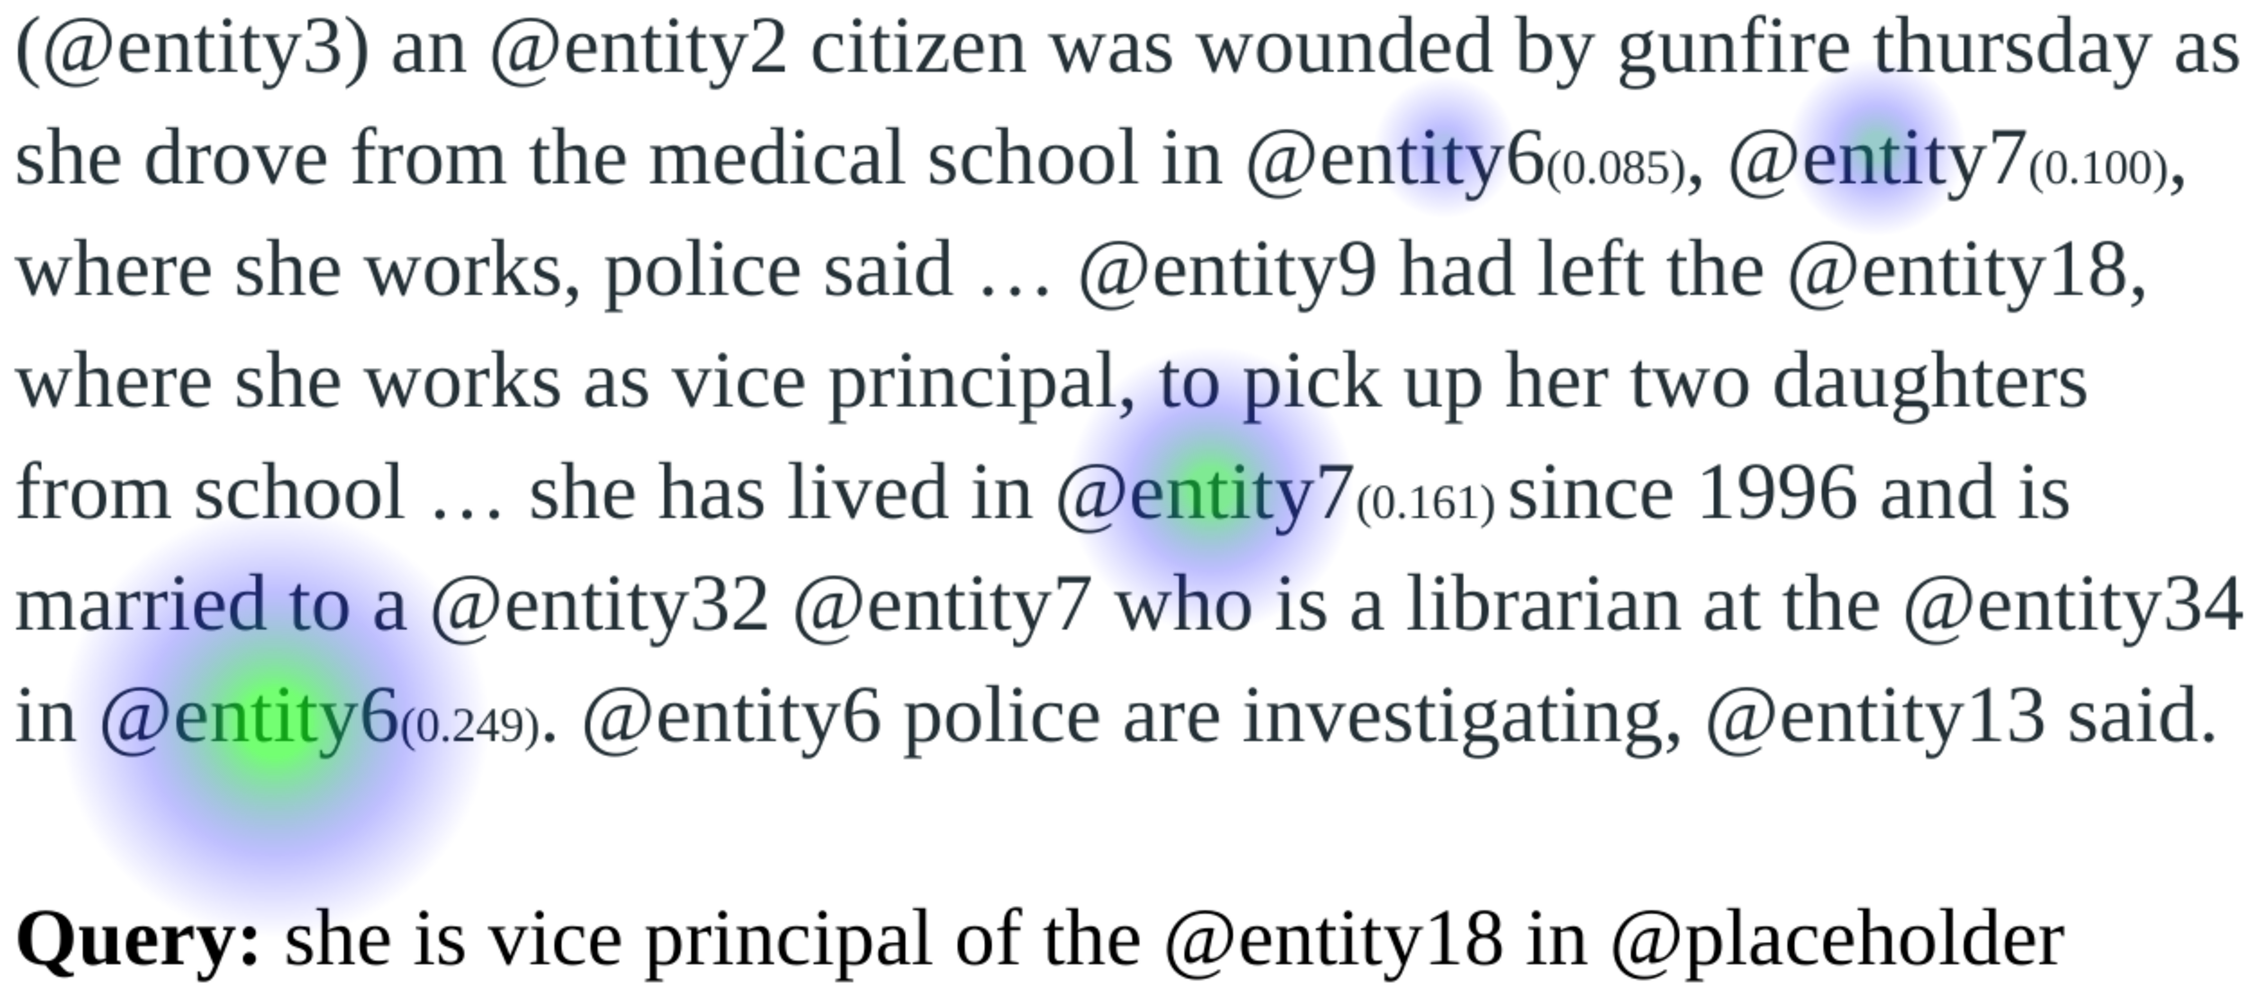
\includegraphics[width=1.0\linewidth]{example1.png}
%         \caption{GA reader correctly answered @entity6.}
%         \label{fig:example1}
%     \end{subfigure}
%     \begin{subfigure}[b]{0.475\textwidth}
%         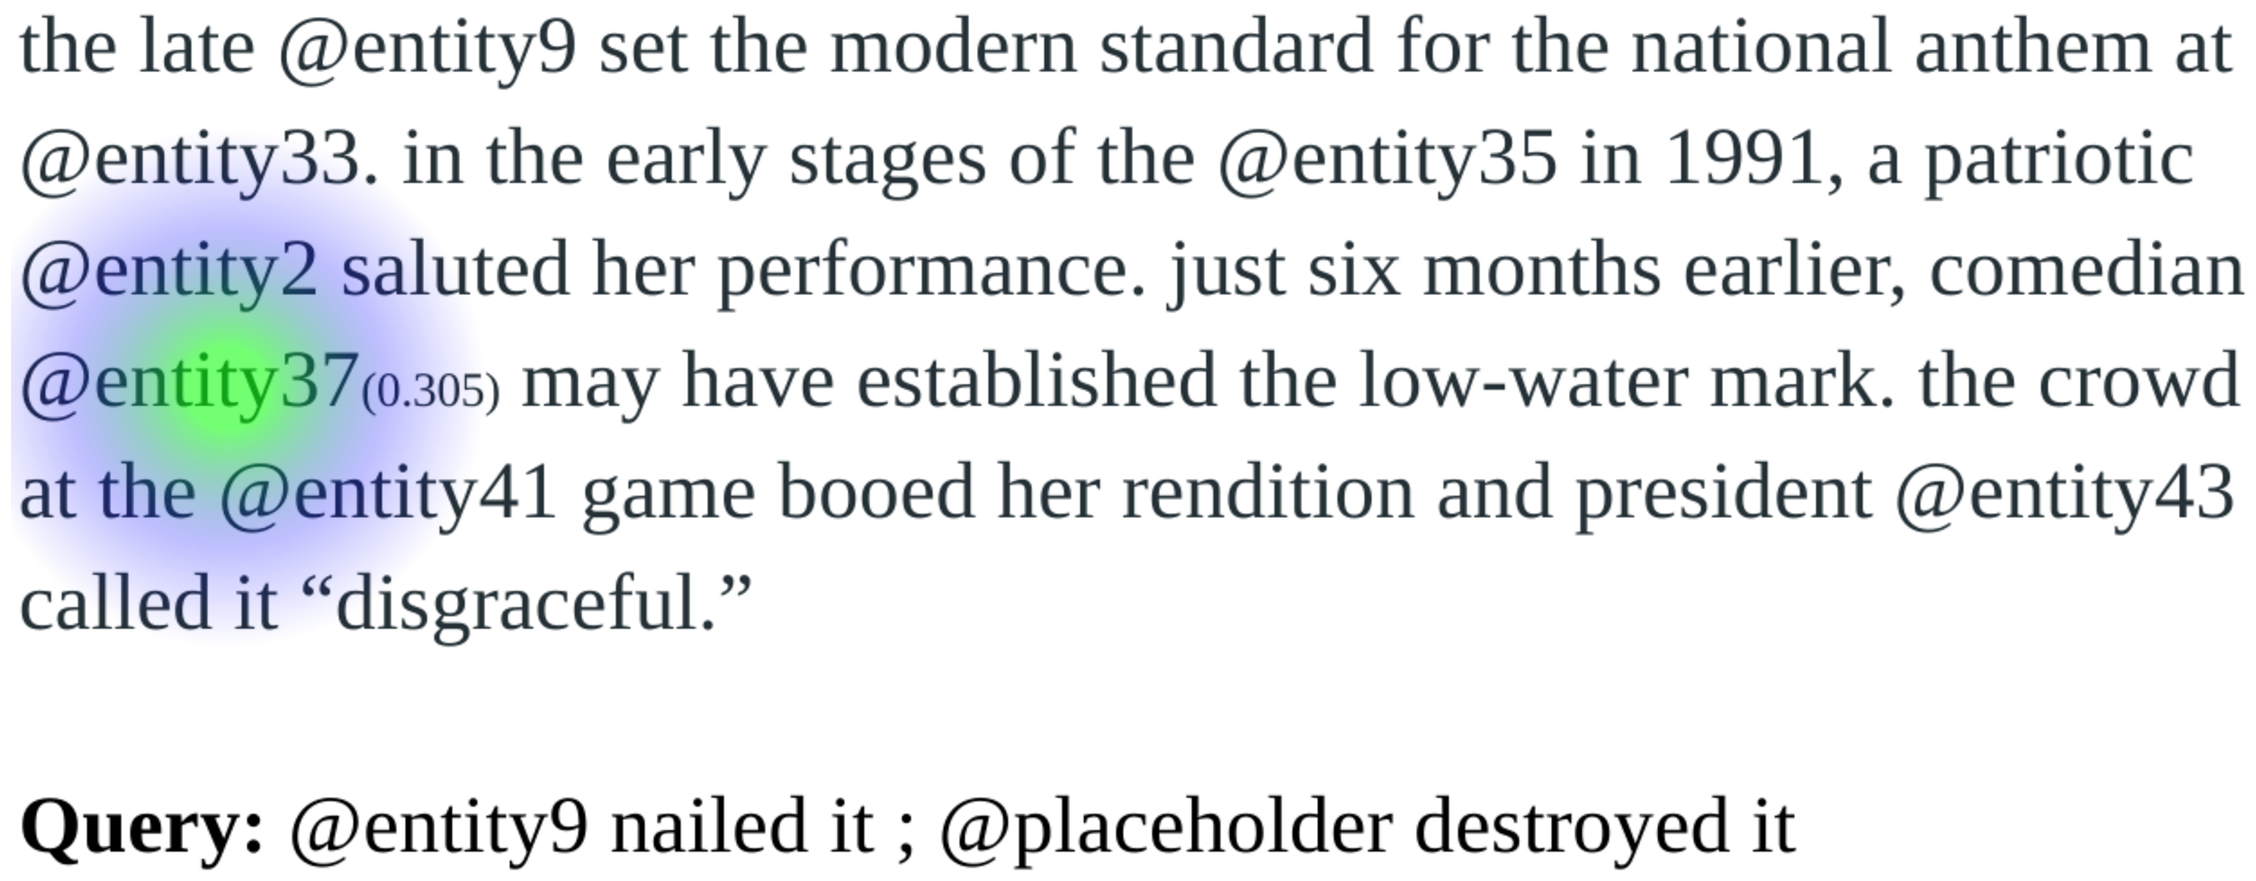
\includegraphics[width=1.0\linewidth]{example2.png}
%         \caption{GA reader correctly answered @entity37.}
%         \label{fig:example2}
%     \end{subfigure}
%     \caption{GA Reader's final-layer attention (before aggregation) over tokens in the questions.}
%     \label{fig:examples}
% \end{figure*}
\subsection{GA Reader Analysis}
\label{sec:ablation}
\begin{figure*}[ht]
    \centering
    \caption{Performance in accuracy with and without the Gated-Attention module over different training sizes. $p$-values for an exact one-sided Mcnemar's test are given inside the parentheses for each setting.}
    \begin{subfigure}[b]{0.245\textwidth}
    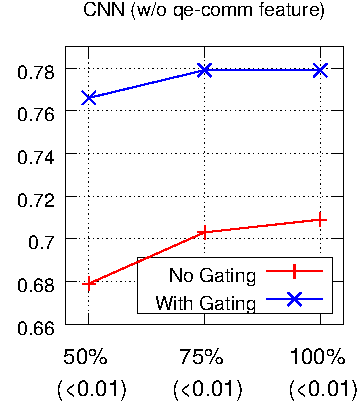
\includegraphics[width=1.0\linewidth]{figures/cnn-feat0-crop}
        \label{fig:cnn_wo_f}
    \end{subfigure}
    \begin{subfigure}[b]{0.245\textwidth}
        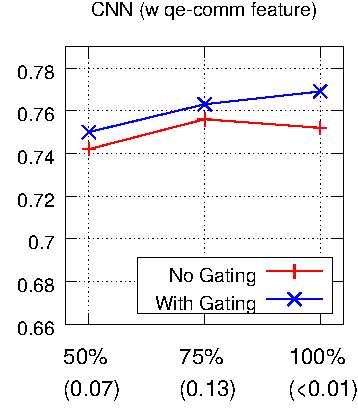
\includegraphics[width=1.0\linewidth]{figures/cnn-feat1-crop}
        \label{fig:cnn_w_f}
    \end{subfigure}
        \begin{subfigure}[b]{0.245\textwidth}
    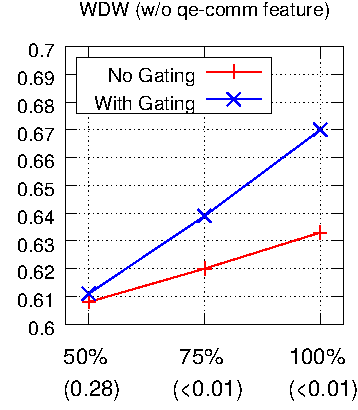
\includegraphics[width=1.0\linewidth]{figures/wdw-feat0-crop}
        \label{fig:wdw_wo_f}
    \end{subfigure}
    \begin{subfigure}[b]{0.245\textwidth}
        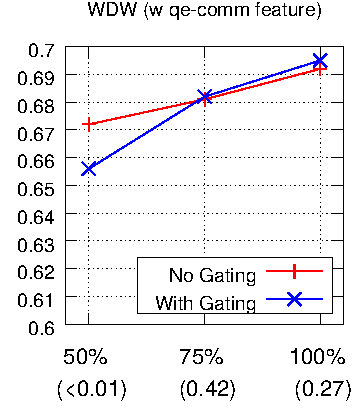
\includegraphics[width=1.0\linewidth]{figures/wdw-feat1-crop}
        \label{fig:wdw_w_f}
    \end{subfigure}
    \label{fig:ablation}
% \vspace{-0.3in}
\end{figure*}

In this section we do an ablation study to see the effect of Gated Attention. We compare the GA Reader as described here to a model which is exactly the same in all aspects, except that it passes document embeddings $D^{(k)}$ in each layer directly to the inputs of the next layer without using the GA module. In other words $X^{(k)}=D^{(k)}$ for all $k>0$. This model ends up using only one query GRU at the output layer for selecting the answer from the document. We compare these two variants both with and without the qe-comm feature on CNN and WDW datasets for three subsets of the training data - 50\%, 75\% and 100\%. Test set accuracies for these settings are shown in Figure~\ref{fig:ablation}. On CNN when tested without feature engineering, we observe that GA provides a significant boost in performance compared to without GA. When tested with the feature it still gives an improvement, but the improvement is significant only with 100\% training data. On WDW-Strict, which is a third of the size of CNN, without the feature we see an improvement when using GA versus without using GA, which becomes significant as the training set size increases. When tested with the feature on WDW, for a small data size without GA does better than with GA, but as the dataset size increases they become equivalent. We conclude that GA provides a boost in the absence of feature engineering, or as the training set size increases.

Next we look at the question of how to gate intermediate document reader states from the query, i.e. what operation to use in equation \ref{eq:gating}. Table ~\ref{tab:gating_fn} (top) shows the performance on WDW dataset for three common choices -- \texttt{sum} ($x=d+q$), \texttt{concatenate} ($x=d \Vert q$) and \texttt{multiply} ($x=d \odot q$). Empirically we find element-wise multiplication does significantly better than the other two, which justifies our motivation to ``filter'' out document features which are irrelevant to the query.

At the bottom of Table~\ref{tab:gating_fn} we show the effect of varying the number of hops $K$ of the GA Reader on the final performance. We note that for $K=1$, our model is equivalent to the AS Reader without any GA modules. We see a steep and steady rise in accuracy as the number of hops is increased from $K=1$ to $3$, which remains constant beyond that. This is a common trend in machine learning as model complexity is increased, however we note that a multi-hop architecture is important to achieve a high performance for this task, and provide further evidence for this in the next section.

% \end{wraptable}
\subsection{Ablation Study for Model Components}
\label{app:ablation}
Table~\ref{tab:ablation} shows accuracy on WDW by removing one component at a time.
\begin{table}[!htbp]
\centering
\caption{\small Ablation study on WDW dataset, without using the qe-comm feature and with fixed $L(w)$. Results marked with $\dagger$ are cf \citet{onishi2016did}.}
\label{tab:ablation}
\begin{tabular}{@{}l|c|c@{}}
\toprule
\multirow{2}{*}{\textbf{Model}} & \multicolumn{2}{c}{\textbf{Accuracy}} \\ \cmidrule(l){2-3} 
                                          & Val                & Test              \\ \midrule
GA                                       & \textbf{68.3}               & \textbf{68.0}             \\
\quad $-$char                               & 66.9               & 66.9              \\
\quad $-$token-attentions (eq. \ref{eq:q_att})  & 65.7               & 65.0              \\
\quad $-$glove, $+$corpus                & 64.0               & 62.5              \\
 \midrule
GA-{}-$\dagger$                & --               & 57              \\ \bottomrule
\end{tabular}
\end{table}
The steepest reduction is observed when we replace pretrained GloVe vectors with those pretrained on the corpus itself. GloVe vectors were trained on a large corpus of about 6 billion tokens \citep{pennington2014glove}, and provide an important source of prior knowledge for the model. Note that the strongest baseline on WDW, NSE~\citep{munkhdalai2016reasoning}, also uses pretrained GloVe vectors, hence the comparison is fair in that respect. Next, we observe a substantial drop when removing token-specific attentions over the query in the GA module, which allow gating individual tokens in the document only by parts of the query relevant to that token rather than the overall query representation. Finally, removing the character embeddings, which were only used for WDW and CBT, leads to a reduction of about 1\% in the performance. 

% Lastly, we perform an ablation study for the three components of the GA Reader which were absent in the preprint version (GA Reader-{}-).
% See Appendix~\ref{app:ablation} for more details.

% \vspace{-0.05in}
\subsection{Attention Visualization}
\begin{figure*}[t]
\centering
\caption{Layer-wise attention visualization of GA Reader trained on WDW-Strict. See text for details.}
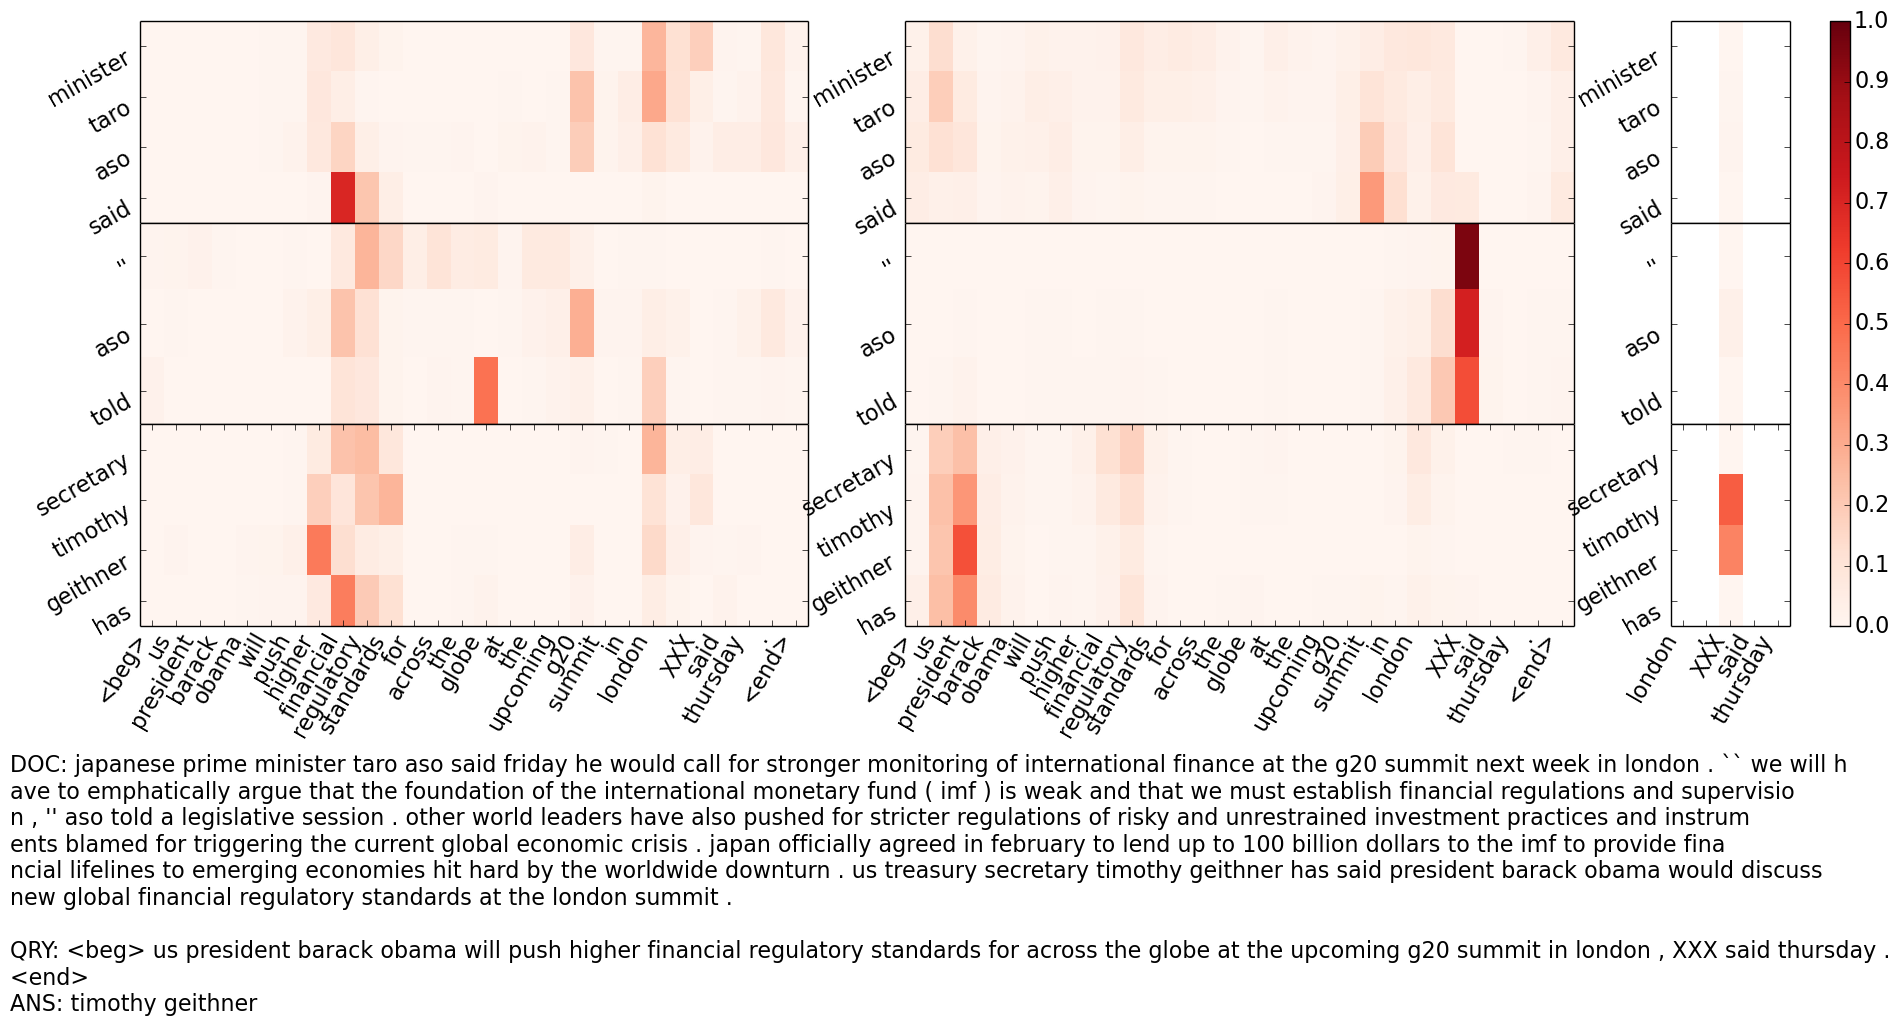
\includegraphics[width=0.91\linewidth]{attention_plots/AFP_ENG_20090326_0419_question.png}
\label{fig:att_plots}
% \vspace{-0.1in}
\end{figure*}

To gain an insight into the reading process employed by the model we analyzed the attention distributions at intermediate layers of the reader.
Figure~\ref{fig:att_plots} shows an example from the validation set of WDW dataset (several more are in the Appendix).
In each figure, the left and middle plots visualize attention over the query (equation~\ref{eq:q_att}) for candidates in the document after layers 1 \& 2 respectively. The right plot shows attention over candidates in the document of cloze placeholder (\texttt{XXX}) in the query at the final layer.
The full document, query and correct answer are shown at the bottom.

A generic pattern observed in these examples is that in intermediate layers,
candidates in the document (shown along rows) tend to pick out salient tokens in the query which provide clues about the cloze, and in the final layer the candidate with the highest match with these tokens is selected as the answer.
In Figure~\ref{fig:att_plots} there is a high attention of the correct answer on \texttt{financial} \texttt{regulatory} \texttt{standards} in the first layer, and on \texttt{us} \texttt{president} in the second layer. The incorrect answer, in contrast, only attends to one of these aspects, and hence receives a lower score in the final layer despite the n-gram overlap it has with the cloze token in the query.
%In the second example, the candidates pick out \texttt{michael} \texttt{llodra}, \texttt{compatriot} and \texttt{partner} in the two layers, all of which are important clues to the correct answer, and the candidate with highest match with these is selected as the answer. The reader picks out these important tokens even when they are far from the cloze in the query.
Importantly, different layers tend to focus on different tokens in the query, supporting the hypothesis that the multi-hop architecture of GA Reader is able to combine distinct pieces of information to answer the query.

% Figure \ref{fig:examples} presents two example questions from the CNN test set with an overlaid heat-map showing the attention at the output layer of the GA reader. The attention is computed as the value of $s_t$ in equation \eqref{eq:att} for each token in the document, and is only visualized when $s_t>0.05$. Both questions require the system to understand paraphrases as well as reason over multiple evidence sentences to arrive at the correct answer. The GA reader manages to attend to the right tokens in both cases.  

% \begin{table*}[t]
% \centering
% \caption{Performance of all models on CNN and Dailymail datasets. Results marked with $^\dagger$ are cf their respective papers. Best single model is in red and best ensemble in blue.}
% \begin{tabular}{c|c|c|c|c}
% \toprule
% \multirow{2}{*}{Model} & \multicolumn{2}{c|}{CNN}      & \multicolumn{2}{c}{Dailymail}\\
%                        & Val Acc (\%) & Test Acc (\%) & Val Acc (\%)  & Test Acc (\%)\\
% \midrule
% Deep LSTM Reader $^\dagger$ & 55.0 & 57.0 & 63.3 & 62.2\\
% Attentive Reader $^\dagger$ & 61.6 & 63.0 & 70.5 & 69.0\\
% Impatient Reader $^\dagger$ & 61.8 & 63.8 & 69.0 & 68.0\\
% \midrule
% Memory Networks (single model) $^\dagger$ & 63.4 & 66.8 & -- & --\\
% Memory Networks (ensemble) $^\dagger$ & 66.2 & 69.4 & -- & --\\
% \midrule
% Attention Sum Reader (single model) $^\dagger$ & 68.6 & 69.5 & 75.0 & 73.9\\
% Attention Sum Reader (ensemble) $^\dagger$ & 73.9 & 75.4 & 78.7 & \blue{\textbf{77.7}}\\
% \midrule
% Dynamic Entity Representations $^\dagger$ & 71.3 & 72.9 & -- & --\\
% \midrule
% Gated-Attention Reader (single model) & 73.0 & \red{\textbf{73.8}} & 76.7 & \red{\textbf{75.7}}\\
% Gated-Attention Reader (ensemble) & 76.4 & \blue{\textbf{77.4}} & 78.6 & 77.6\\
% \bottomrule
% \end{tabular}
% \label{tab:results_cnn_dm}
% \end{table*}

% \begin{table*}[t]
% \centering
% \caption{Performance of all models on CBT datasets. Results marked with $^\dagger$ are cf their respective papers. Best single model is in red, and best ensemble in blue.}
% \begin{tabular}{c|c|c|c|c}
% \toprule
% \multirow{2}{*}{Model} & \multicolumn{2}{c|}{CBT-NE}      & \multicolumn{2}{c}{CBT-CN}\\
%                        & Val Acc (\%) & Test Acc (\%) & Val Acc (\%)  & Test Acc (\%)\\
% \midrule
% Humans (query) $^\dagger$ & -- & 52.0 & -- & 64.4\\
% Humans (context + query) $^\dagger$ & -- & 81.6 & -- & 81.6\\
% \midrule
% LSTMs (context + query) $^\dagger$ & 51.2 & 41.8 & 62.6 & 56.0\\
% \midrule
% Memory Networks (best model) $^\dagger$ & 70.4 & 66.6 & 64.2 & 63.0\\
% \midrule
% Attention Sum Reader (single model) $^\dagger$ & 73.8 & 68.6 & 68.8 & 63.4 \\
% Attention Sum Reader (ensemble) $^\dagger$ & 76.2 & 71.0 & 71.1 & 68.9\\
% \midrule
% Gated-Attention Reader (single model) & 74.9 & \red{\textbf{69.0}} & 69.0 & \red{\textbf{63.9}} \\
% Gated-Attention Reader (ensemble) & 75.5 & \blue{\textbf{71.9}} & 72.1 & \blue{\textbf{69.4}}\\
% \bottomrule
% \end{tabular}
% \label{tab:results_cbt}
% \end{table*}

\section{Conclusion}
\label{sec:conclusion}
We presented the Gated-Attention reader for answering cloze-style questions over documents.
The GA reader features a novel multiplicative gating mechanism, combined with a multi-hop architecture.
Our model achieves the state-of-the-art performance on several large-scale benchmark datasets with more than 4\% improvements over competitive baselines. Our model design is backed up by an ablation study showing statistically significant improvements of using Gated Attention as information filters. We also showed empirically that multiplicative gating is superior to addition and concatenation operations for implementing gated-attentions, though a theoretical justification remains part of future research goals. Analysis of document and query attentions in intermediate layers of the reader further reveals that the model iteratively attends to different aspects of the query to arrive at the final answer. In this paper we have focused on text comprehension, but we believe that the Gated-Attention mechanism may benefit other tasks as well where multiple sources of information interact.
% Concurrent to our work \citep{chu2016broad} have also shown the effectiveness of GA Readers on the LAMBADA dataset \citep{paperno2016lambada} for language modeling.

% \begin{table}
% \centering
% \begin{tabular}{@{}c|cccc@{}}
% \toprule
% \textbf{Features} & \textbf{WD} & \textbf{LSTM} & \textbf{AS} & \textbf{GA} \\ \midrule
% \texttt{DL}     &   \underline{-1.43}        & \underline{-1.73}         & -0.42       & -1.18       \\
% \texttt{QL}     &   -0.37       & -0.08         & -0.28       & -0.12       \\
% \texttt{AF}     &   \underline{0.73}        & 0.50          & 0.53        & 0.30        \\
% \texttt{AFL}    &   -0.14        & \underline{-0.71}         & -0.36       & \underline{-0.47}       \\
% \texttt{ALL}    &   0.24        & 0.10          & -0.16       & -0.12       \\
% \texttt{ES}     &   -0.07        & -0.02         & -0.33       & -0.05       \\
% \texttt{NG}     &   0.15        & 0.10          & 0.02        & 0.15        \\
% \texttt{P}      &   \underline{-0.33}        & -0.10         & \underline{-0.29}       & -0.10       \\
% \texttt{LR}     &   -0.01        & -0.18         & 0.11        & 0.02        \\
% \texttt{TR}     &   -0.25        & -0.18         & -0.04       & -0.24       \\ \bottomrule
% \end{tabular}
% \caption{Regression coefficients of linguistic features. A positive value indicates a positive effect on the model's test-set performance and vice versa. Coefficients that are statistically significant under $5\%$ level are underlined.}
% \end{table}


\section*{Acknowledgments}
% We would like to thank Eduard Hovy and Teruko Mitamura for useful comments on this work. 
This work was funded by NSF under CCF1414030 and Google Research.

\bibliography{iclr2017_conference}
\bibliographystyle{iclr2017_conference}

\appendix

\vspace{-0.05in}
\section{Implementation Details}
\label{app:implementation}
\begin{table*}[t]
\centering
\caption{\small Dataset statistics.}
\label{tab:data}
\begin{tabular}{@{}crrrrrr@{}}
\toprule
 & \textbf{CNN} & \textbf{Daily Mail} & \textbf{CBT-NE} & \textbf{CBT-CN} & \textbf{WDW-Strict} & \textbf{WDW-Relaxed} \\ \midrule
\# train              & 380,298             & 879,450               & 108,719              & 120,769  & 	 127,786	&	185,978           \\
\# validation        & 3,924             & 64,835              & 2,000             & 2,000  	&	10,000	&	10,000           \\
\# test           &  3,198            & 53,182               & 2,500              & 2,500  	&	10,000	&	10,000            \\
\# vocab           & 118,497             & 208,045               & 53,063              & 53,185 	&	347,406	&	 308,602             \\ 
max doc length	& 2,000	&	2,000 &	1,338 &	1,338 & 3,085	&	3,085 \\ \bottomrule
\end{tabular}
\end{table*}

\begin{table*}[t]
\centering
\caption{\small Hyperparameter settings for each dataset. dim() indicates hidden state size of GRU.}
\label{tab:params}
\begin{tabular}{@{}ccccccc@{}}
\toprule
\textbf{Hyperparameter} & \textbf{CNN} & \textbf{Daily Mail} & \textbf{CBT-NE} & \textbf{CBT-CN} & \textbf{WDW-Strict} & \textbf{WDW-Relaxed} \\ \midrule
%\# Layers ($K$)	&	3	&	3	&	3	&	3	&	3	&	3	\\
Dropout	&	0.2	&	0.1	&	0.4	&	0.4	&	0.3	&	0.3	\\
$\mathrm{dim}(\bigru_*)$ &	256	&	256	&	128	&	128	&	128	&	128	\\ \bottomrule
%dim($\phi_C$)	&	--	&	--	&	50	&	50	&	50	&	50	\\ \bottomrule
\end{tabular}
\end{table*}

Our model was implemented using the Theano \citep{2016arXiv160502688short} and Lasagne\footnote{\scriptsize \url{https://lasagne.readthedocs.io/en/latest/}} Python libraries. We used stochastic gradient descent with ADAM updates for optimization, which combines classical momentum and adaptive gradients \citep{kingma2014adam}. The batch size was 32 and the initial learning rate was $5\times 10^{-4}$ which was halved every epoch after the second epoch.
The same setting is applied to all models and datasets. We also used gradient clipping with a threshold of 10 to stabilize GRU training \citep{pascanu2012difficulty}.
We set the number of layers $K$ to be $3$ for all experiments.
The number of hidden units for the character GRU was set to 50.
The remaining two hyperparameters---size of document and query GRUs, and dropout rate---were tuned on the validation set, and their optimal values are shown in Table~\ref{tab:params}. In general, the optimal GRU size increases and the dropout rate decreases as the corpus size increases.

The word lookup table was initialized with $100d$ GloVe vectors\footnote{\scriptsize \url{http://nlp.stanford.edu/projects/glove/}} \citep{pennington2014glove} and OOV tokens at test time were assigned unique random vectors. We empirically observed that initializing with pre-trained embeddings gives higher performance compared to random initialization for all datasets. Furthermore, for smaller datasets (WDW and CBT) we found that fixing these embeddings to their pretrained values led to higher test performance, possibly since it avoids overfitting. We do not use the character composition model for CNN and Daily Mail, since their entities (and hence candidate answers) are anonymized to generic tokens. For other datasets the character lookup table was randomly initialized with $25d$ vectors. All other parameters were initialized to their default values as specified in the Lasagne library.


\section{Attention Plots}
\begin{figure*}[h]
\centering
\caption{Layer-wise attention visualization of GA Reader trained on WDW-Strict. See text for details.}
\begin{subfigure}[b]{\textwidth}
\centering
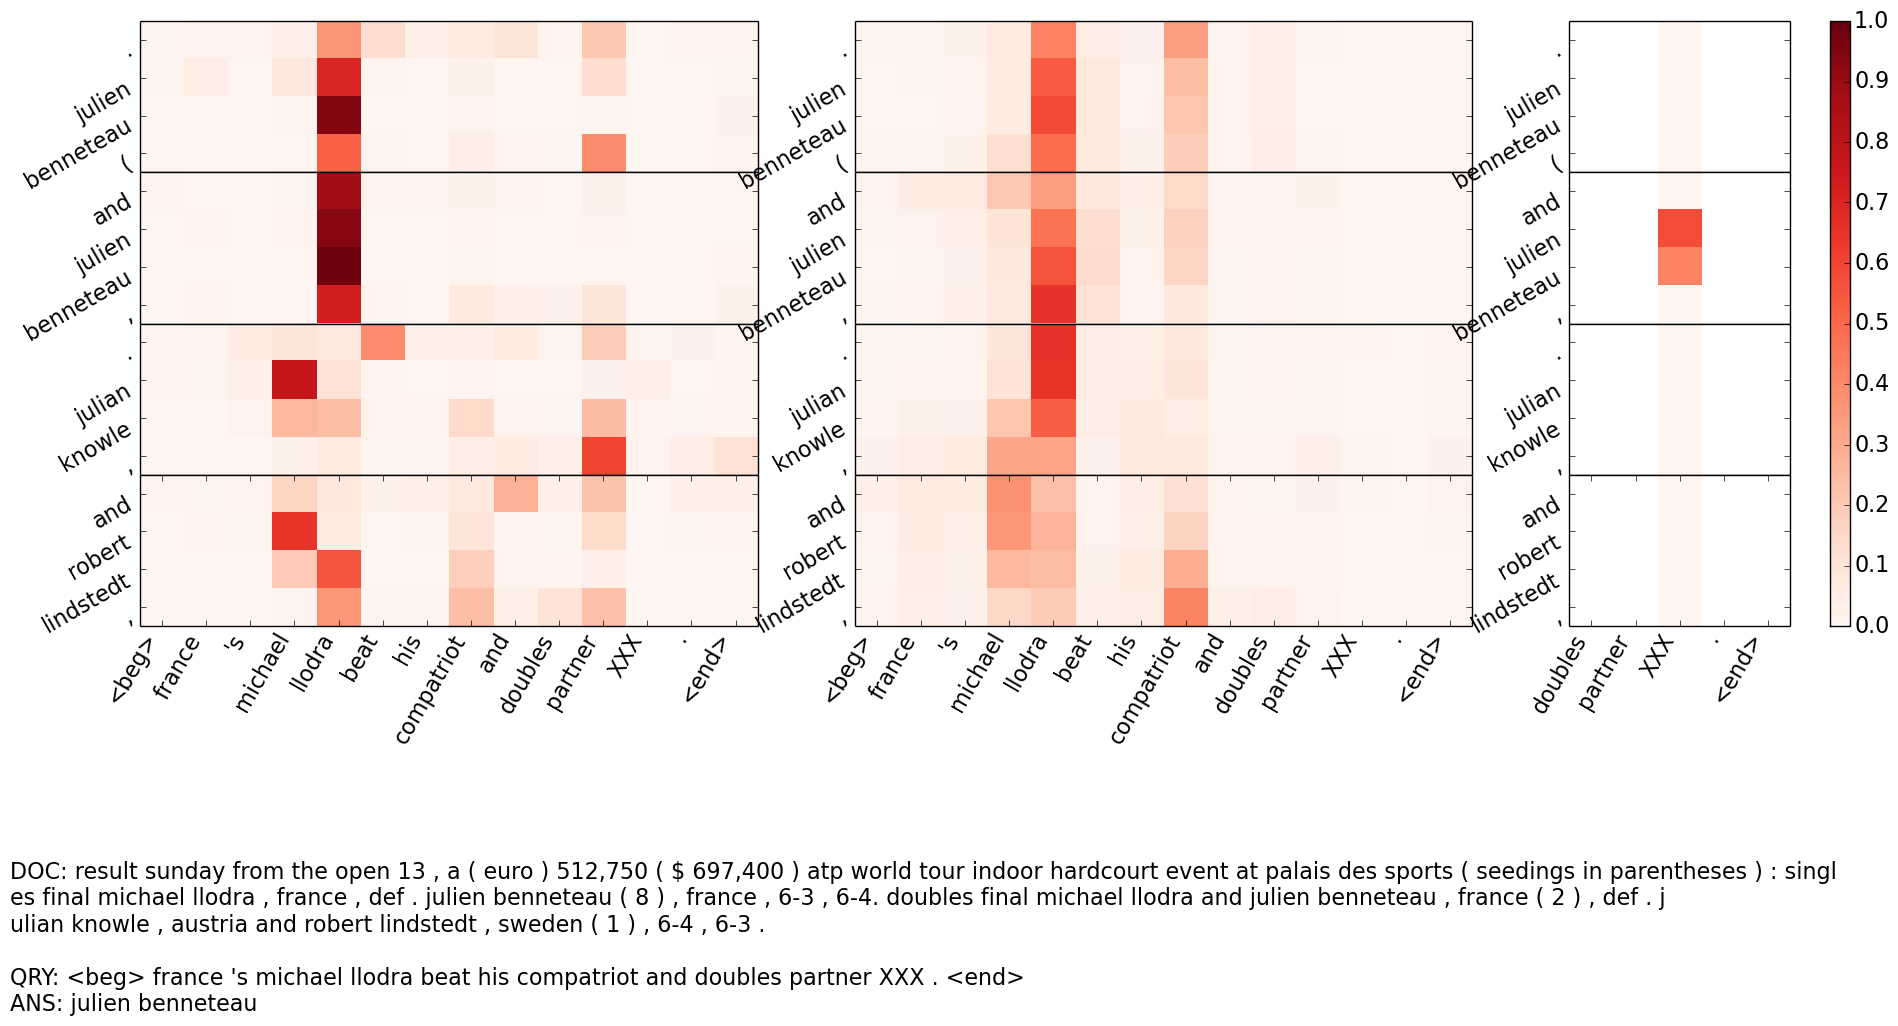
\includegraphics[width=\linewidth]{attention_plots/AFP_ENG_20100221_0186_question.png}
\end{subfigure}
\begin{subfigure}[b]{\textwidth}
\centering
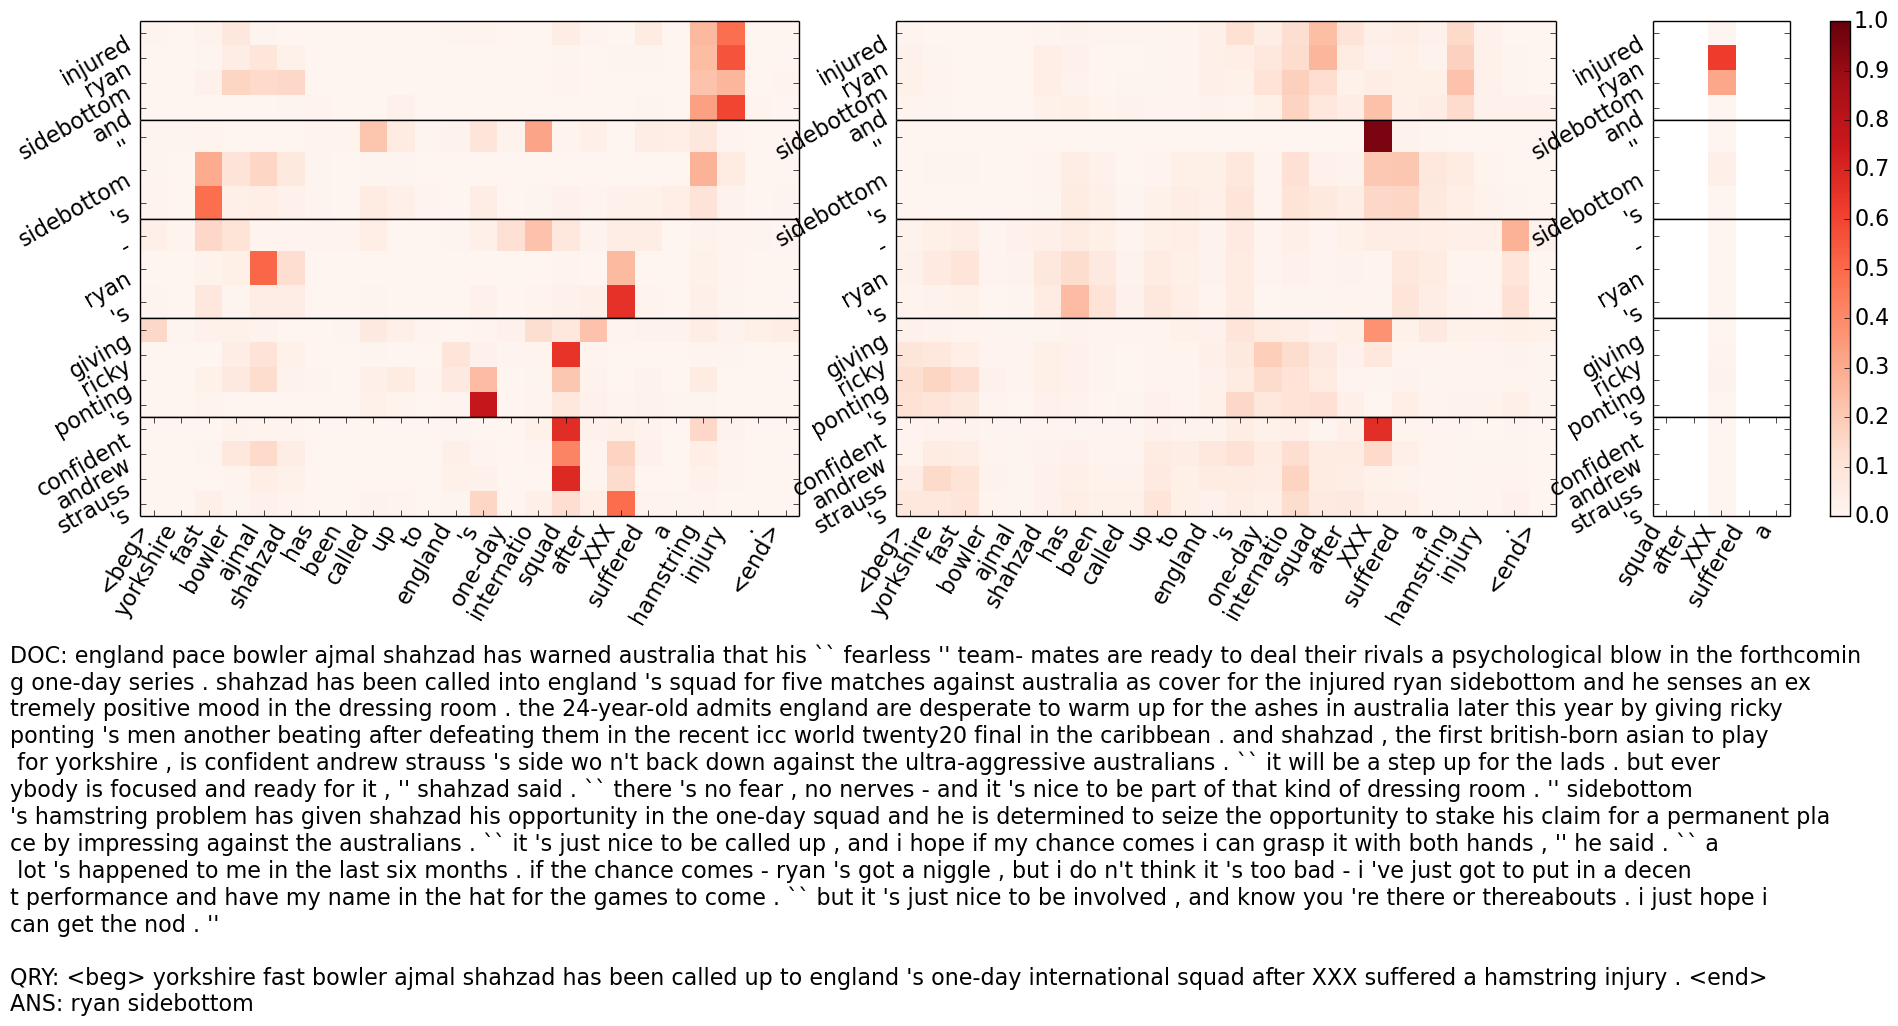
\includegraphics[width=\linewidth]{attention_plots/APW_ENG_20100615_0750_question.png}
\end{subfigure}
\end{figure*}

\begin{figure*}[h]
\centering
\caption{Layer-wise attention visualization of GA Reader trained on WDW-Strict. See text for details.}
\begin{subfigure}[b]{\textwidth}
\centering
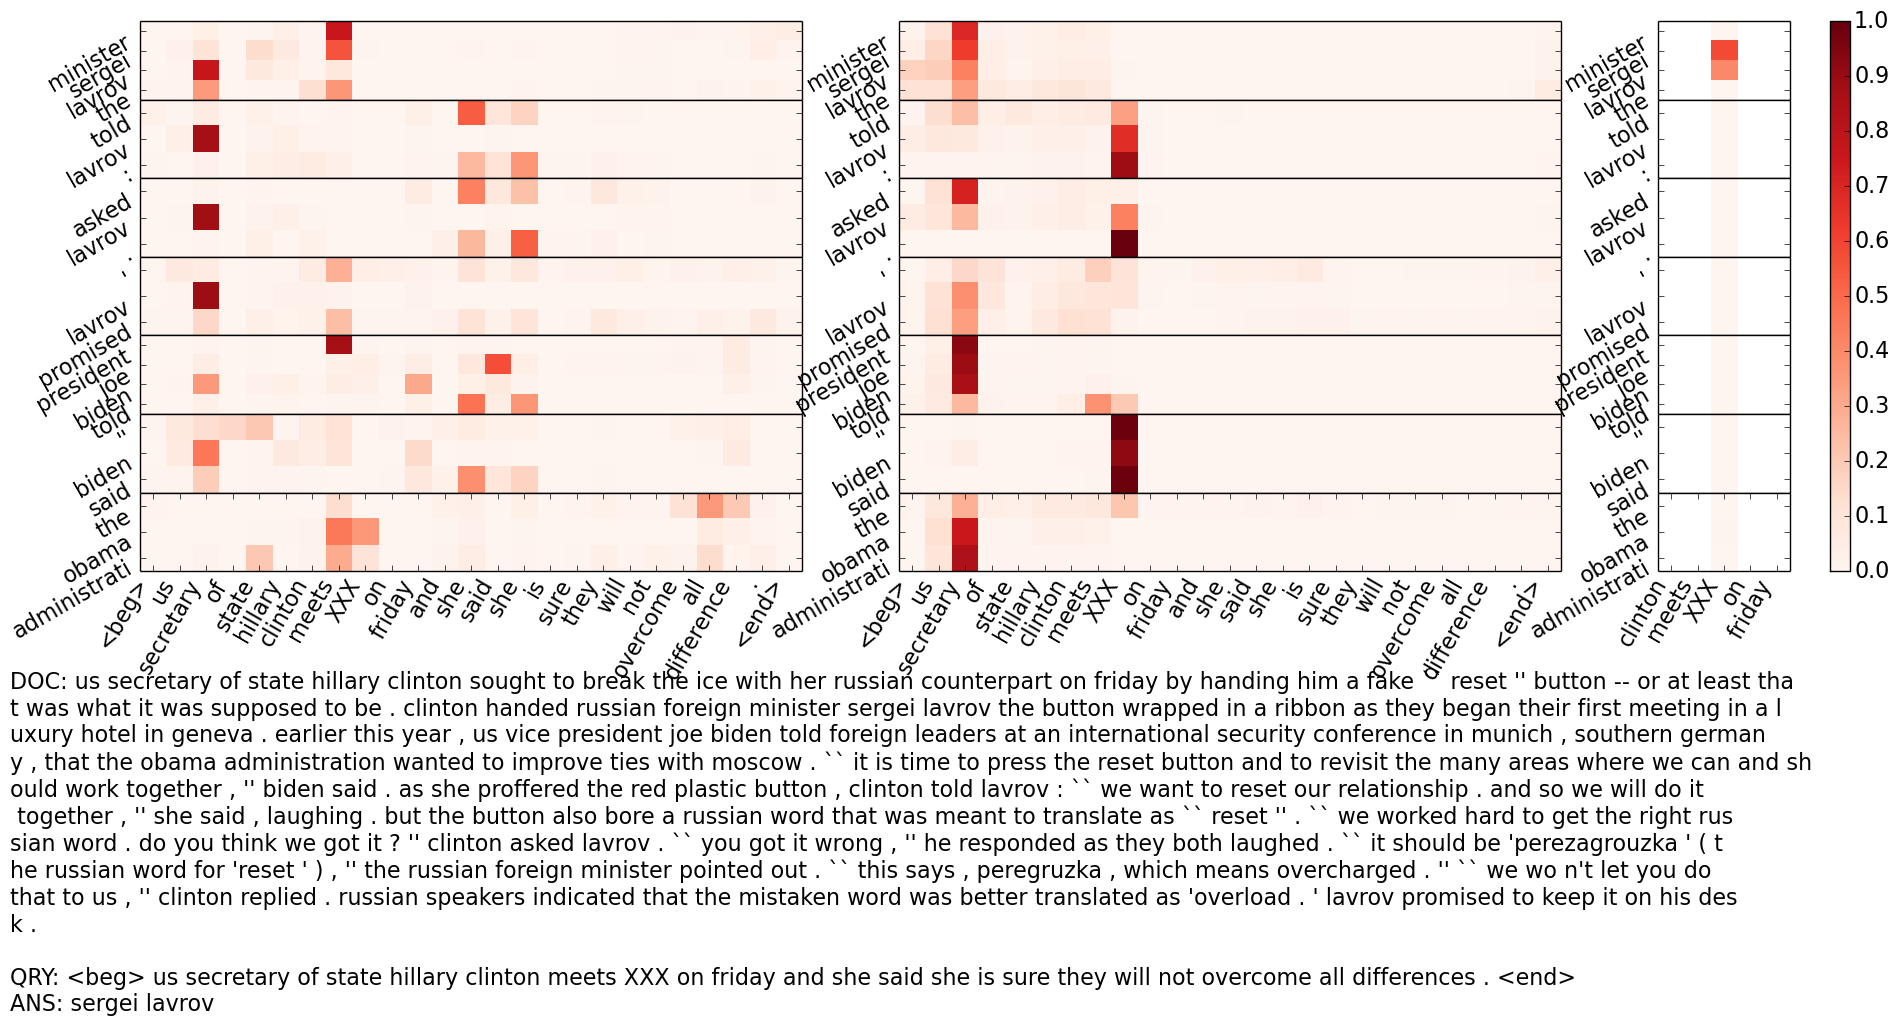
\includegraphics[width=\linewidth]{attention_plots/AFP_ENG_20090306_0553_question.png}
\end{subfigure}
\begin{subfigure}[b]{\textwidth}
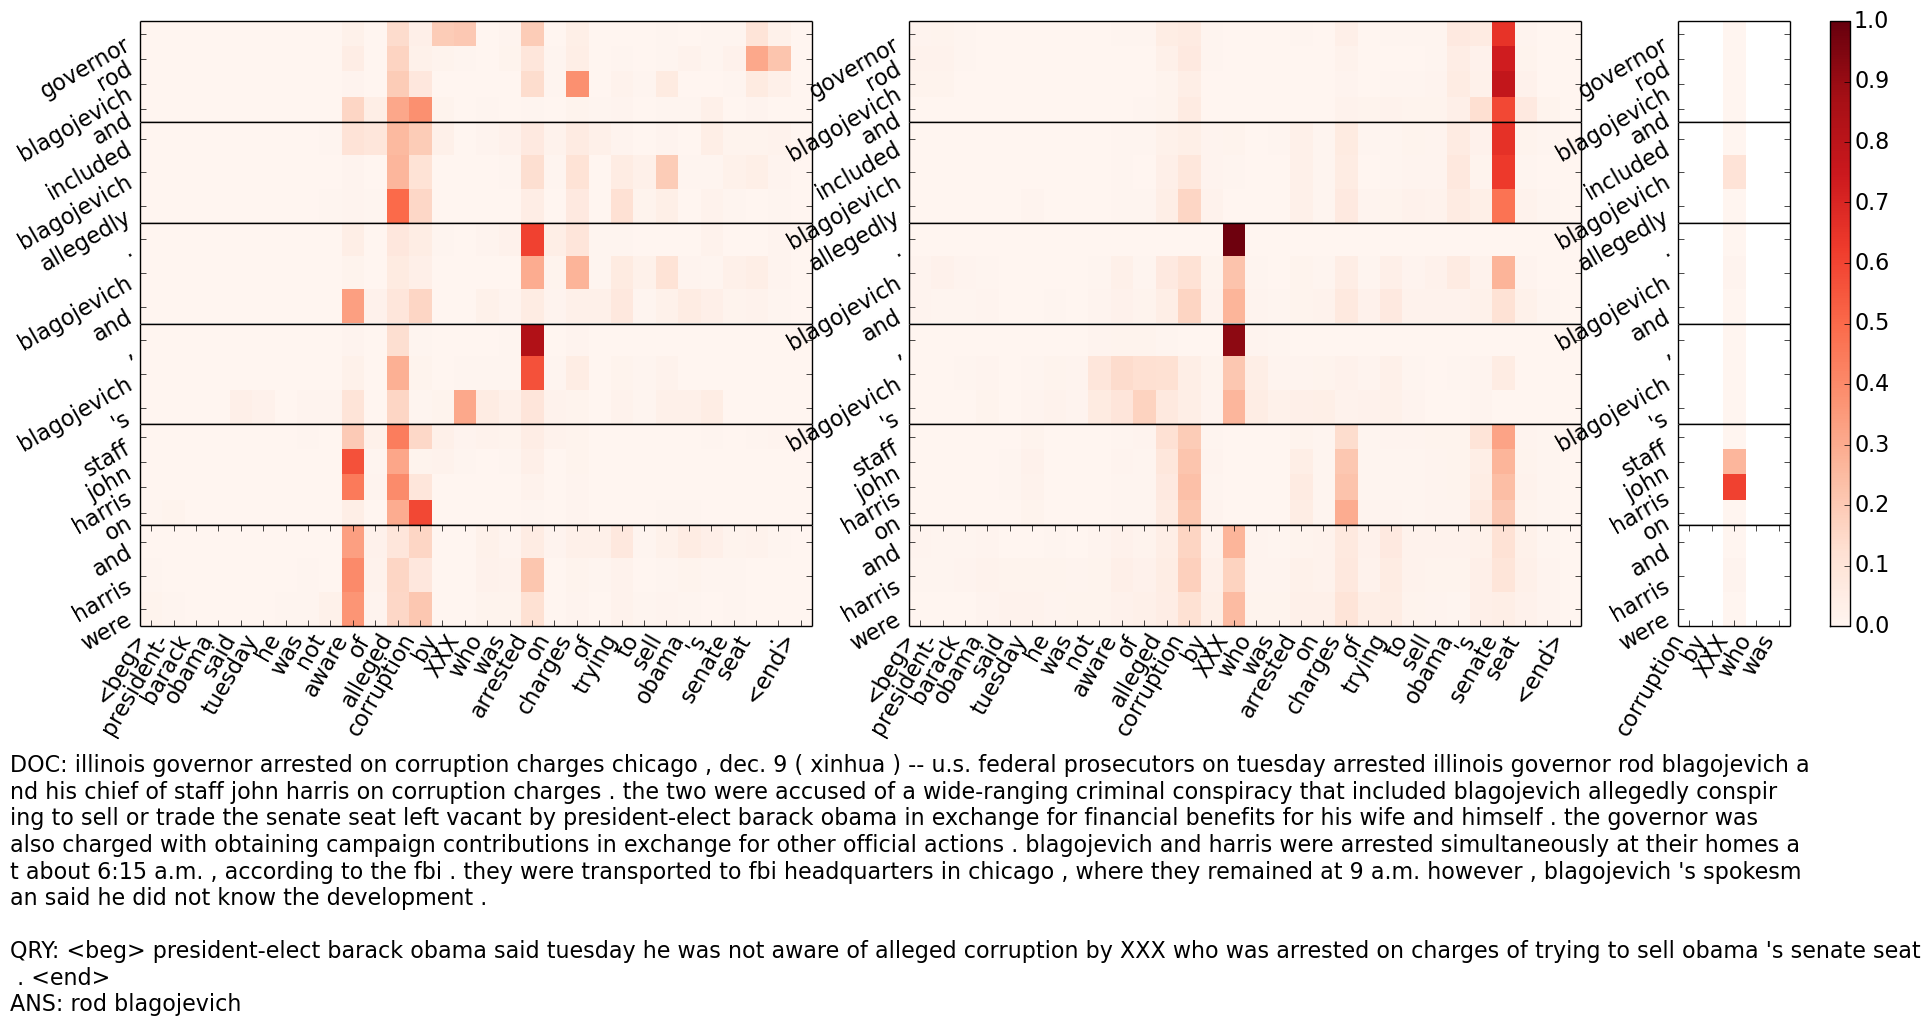
\includegraphics[width=\linewidth]{attention_plots/AFP_ENG_20081210_0707_question.png}
\end{subfigure}
\end{figure*}

\begin{figure*}
\centering
\caption{\small Layer-wise attention visualization of GA Reader trained on WDW-Strict. See text for details.}
\begin{subfigure}[b]{\textwidth}
\centering
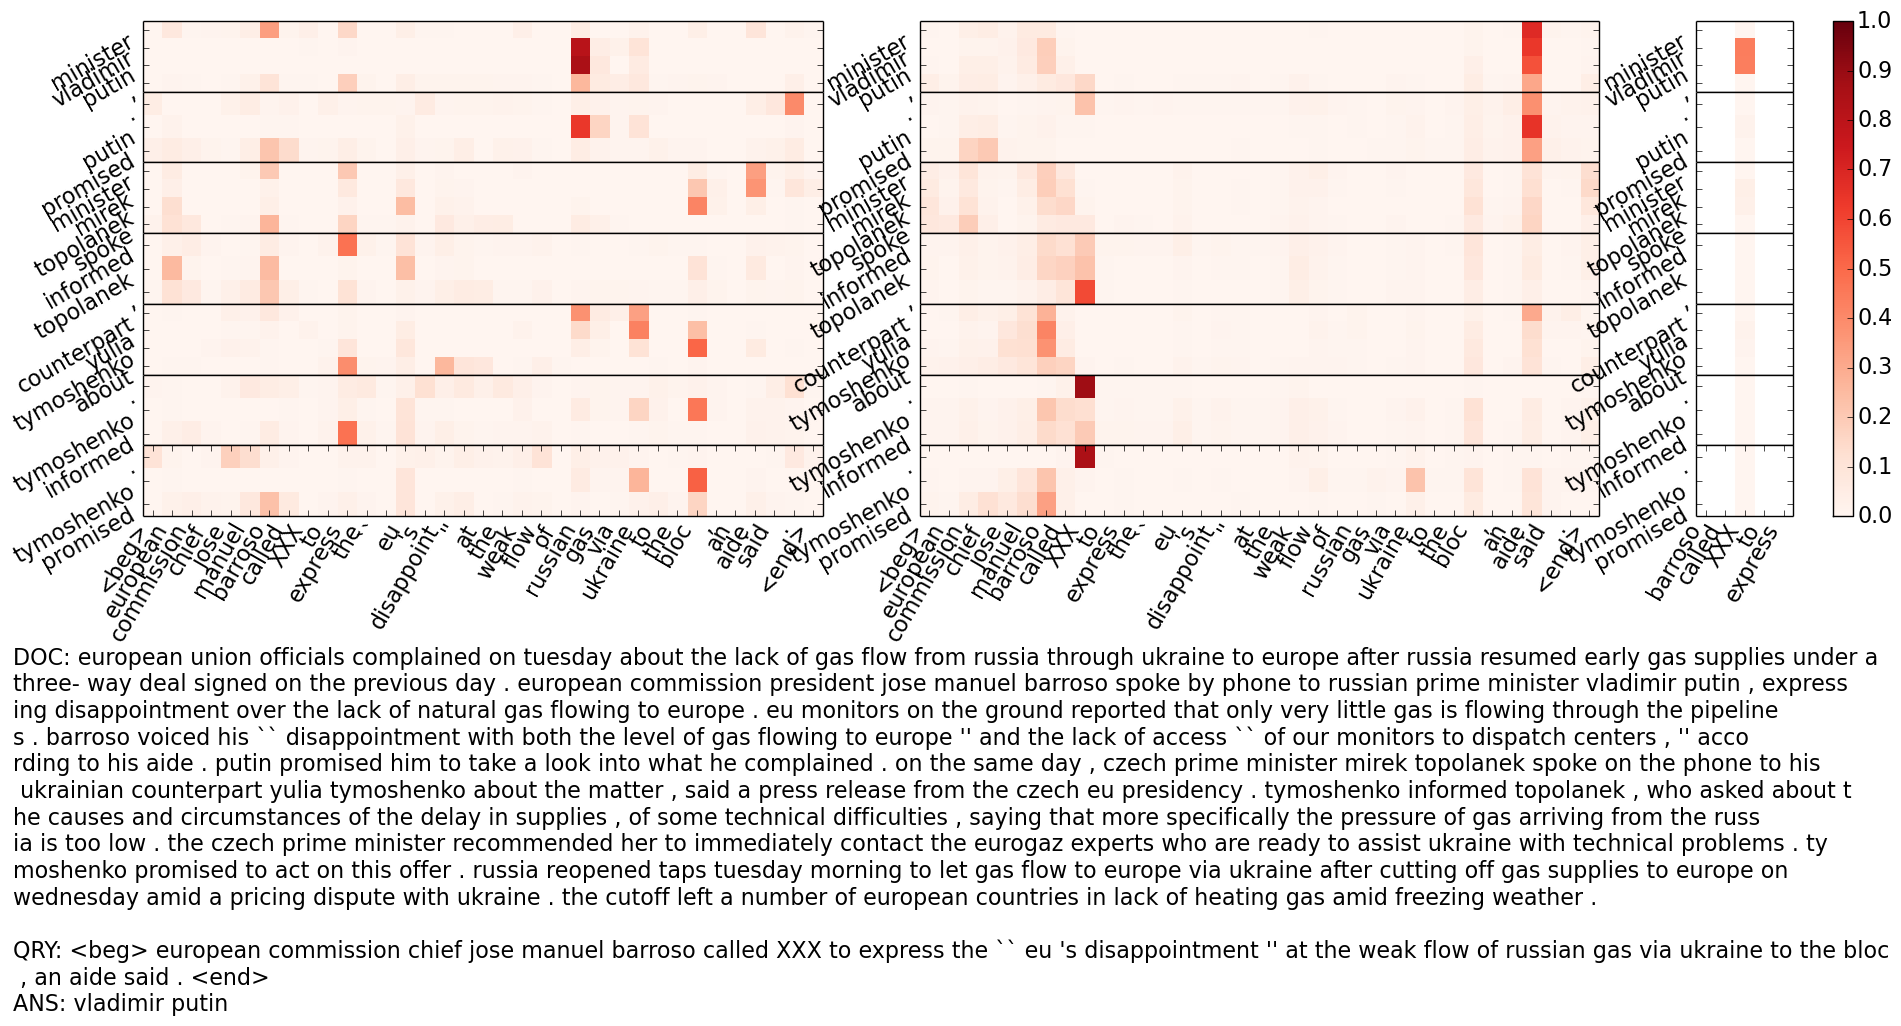
\includegraphics[width=\linewidth]{attention_plots/AFP_ENG_20090113_0407_question.png}
\end{subfigure}
\begin{subfigure}[b]{\textwidth}
\centering
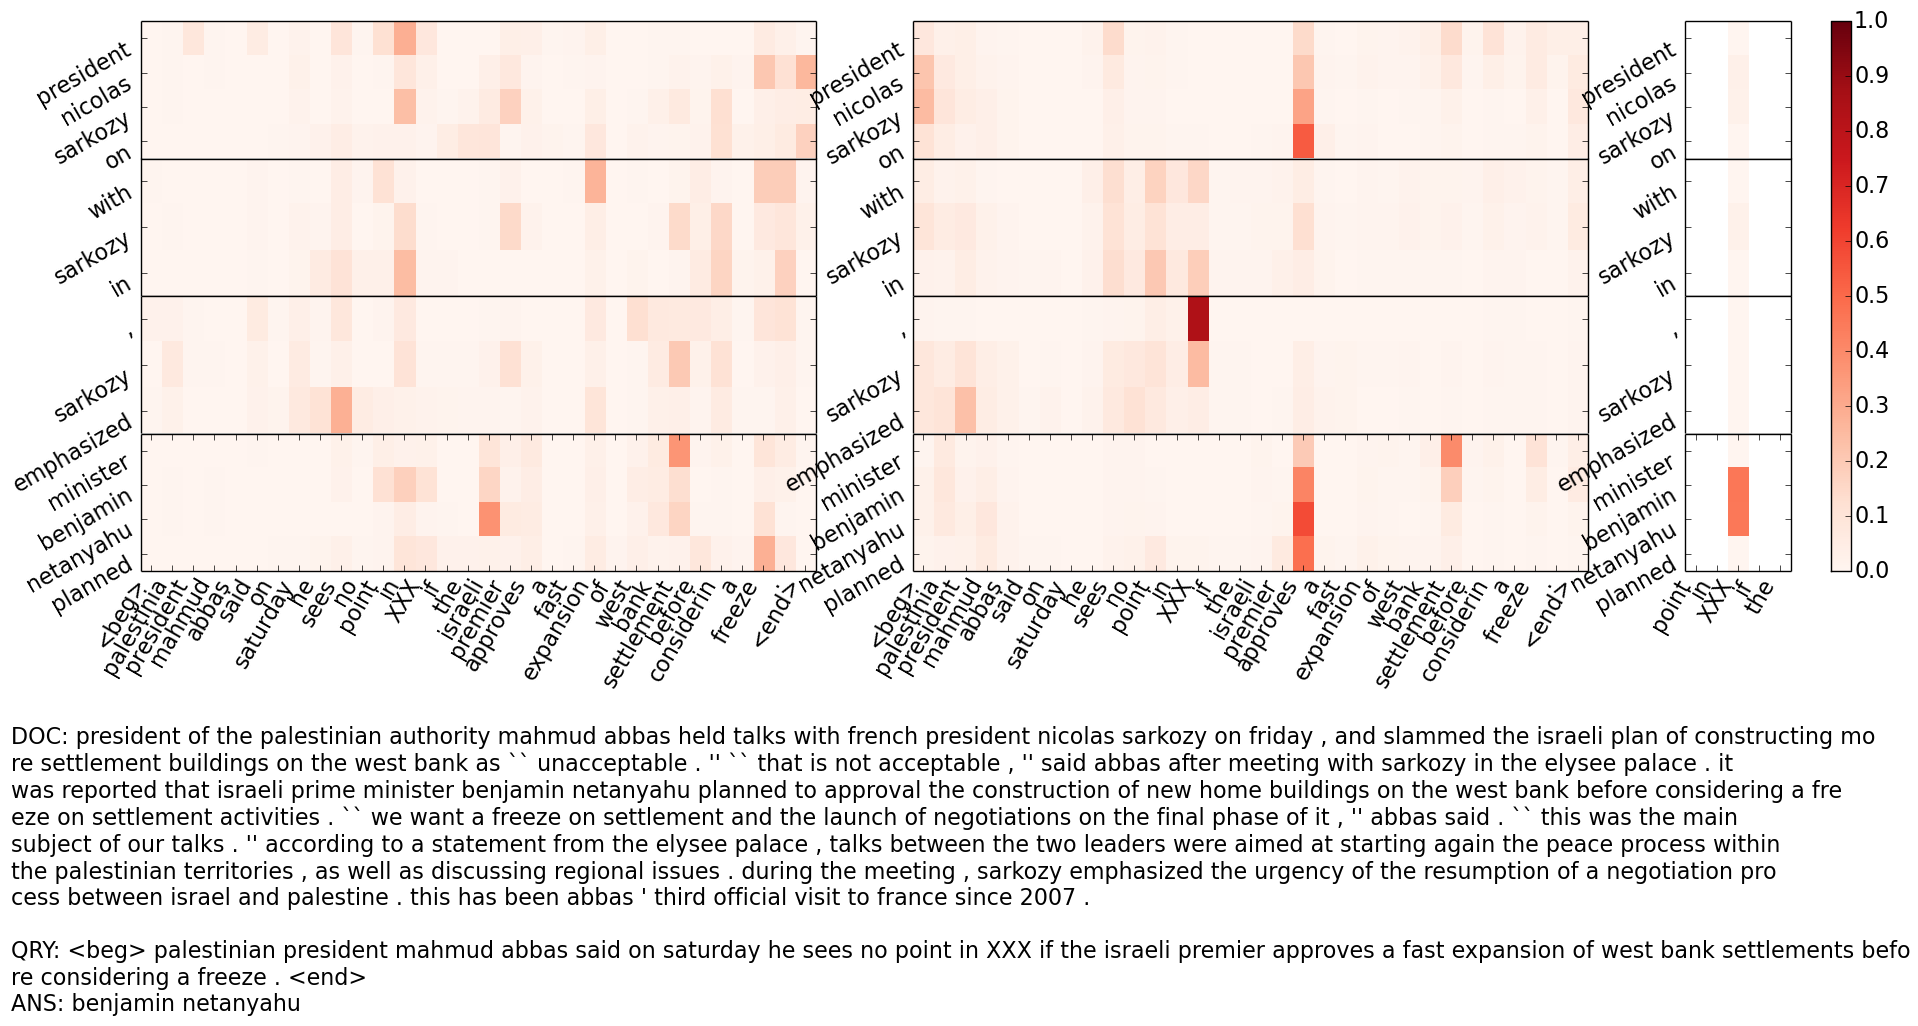
\includegraphics[width=\linewidth]{attention_plots/AFP_ENG_20090905_0240_question.png}
\end{subfigure}
\end{figure*}

\begin{figure*}
\centering
\caption{\small Layer-wise attention visualization of GA Reader trained on WDW-Strict. See text for details.}
\begin{subfigure}[b]{\textwidth}
\centering
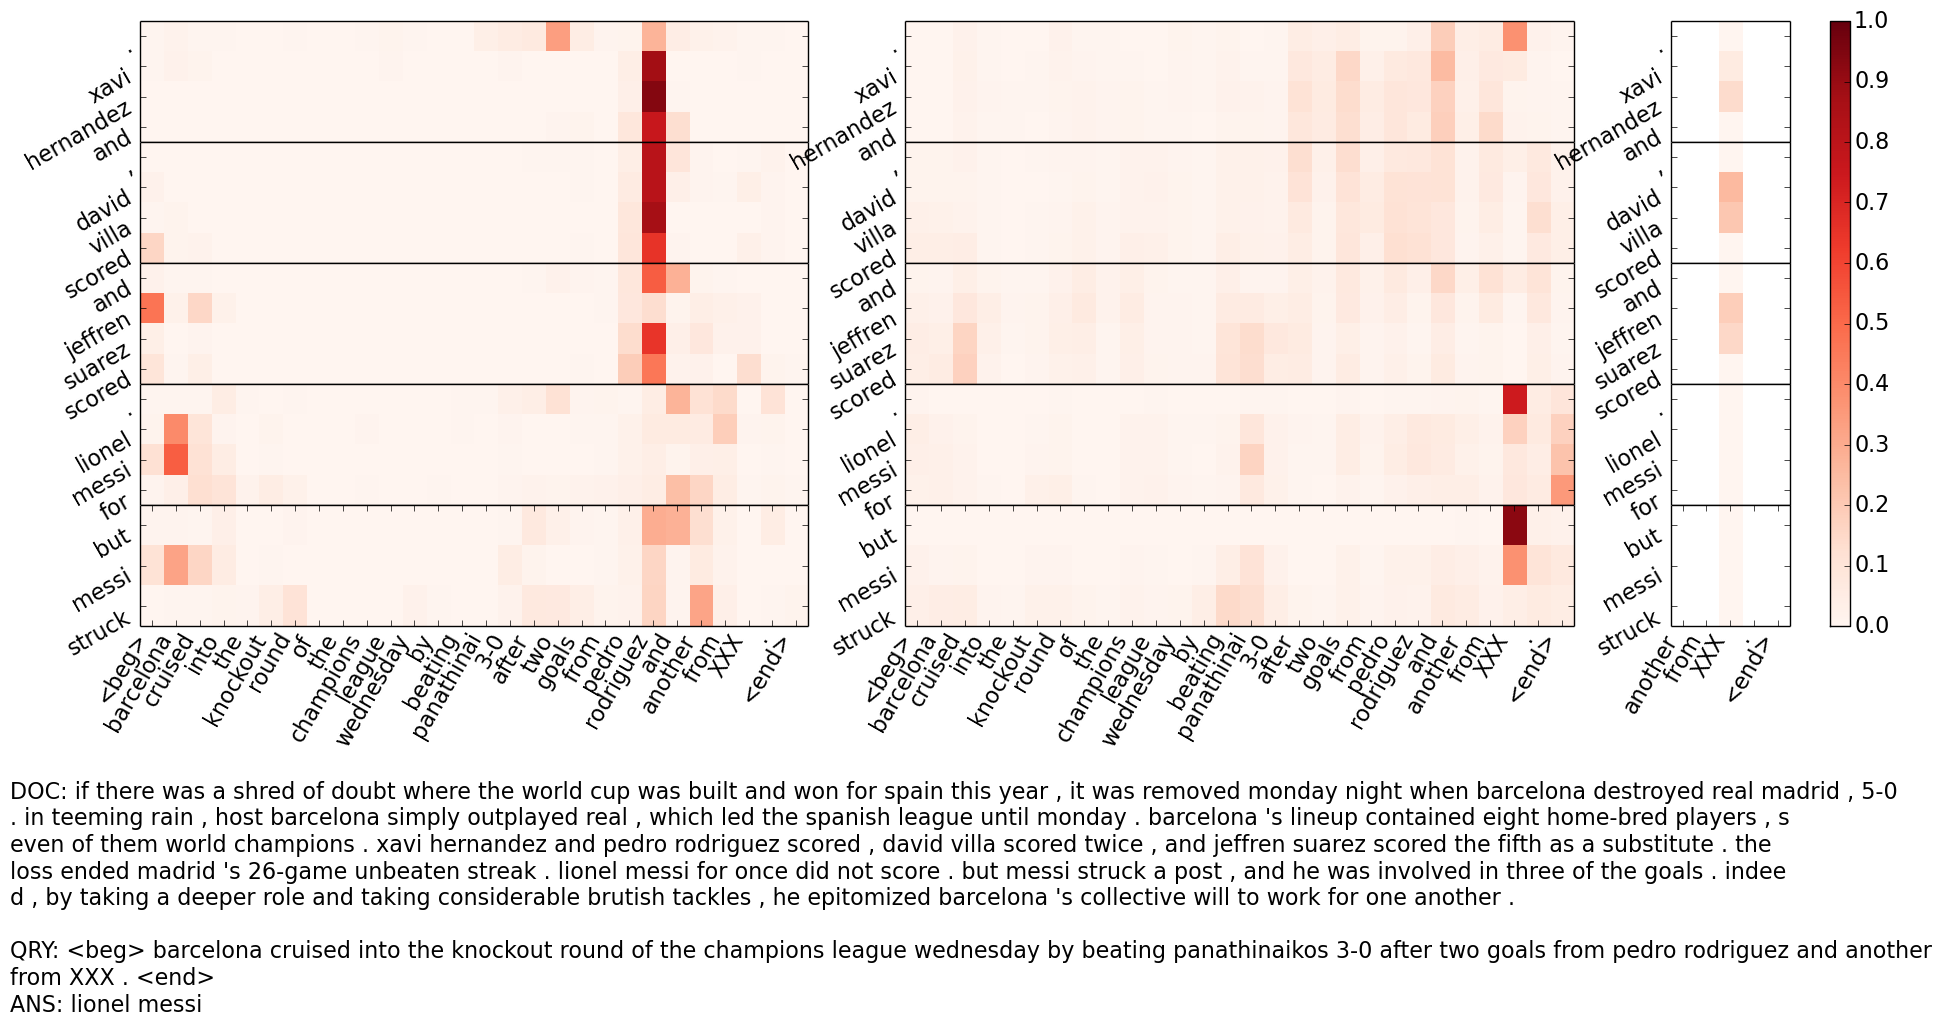
\includegraphics[width=\linewidth]{attention_plots/APW_ENG_20101124_0890_question.png}
\end{subfigure}
\begin{subfigure}[b]{\textwidth}
\centering
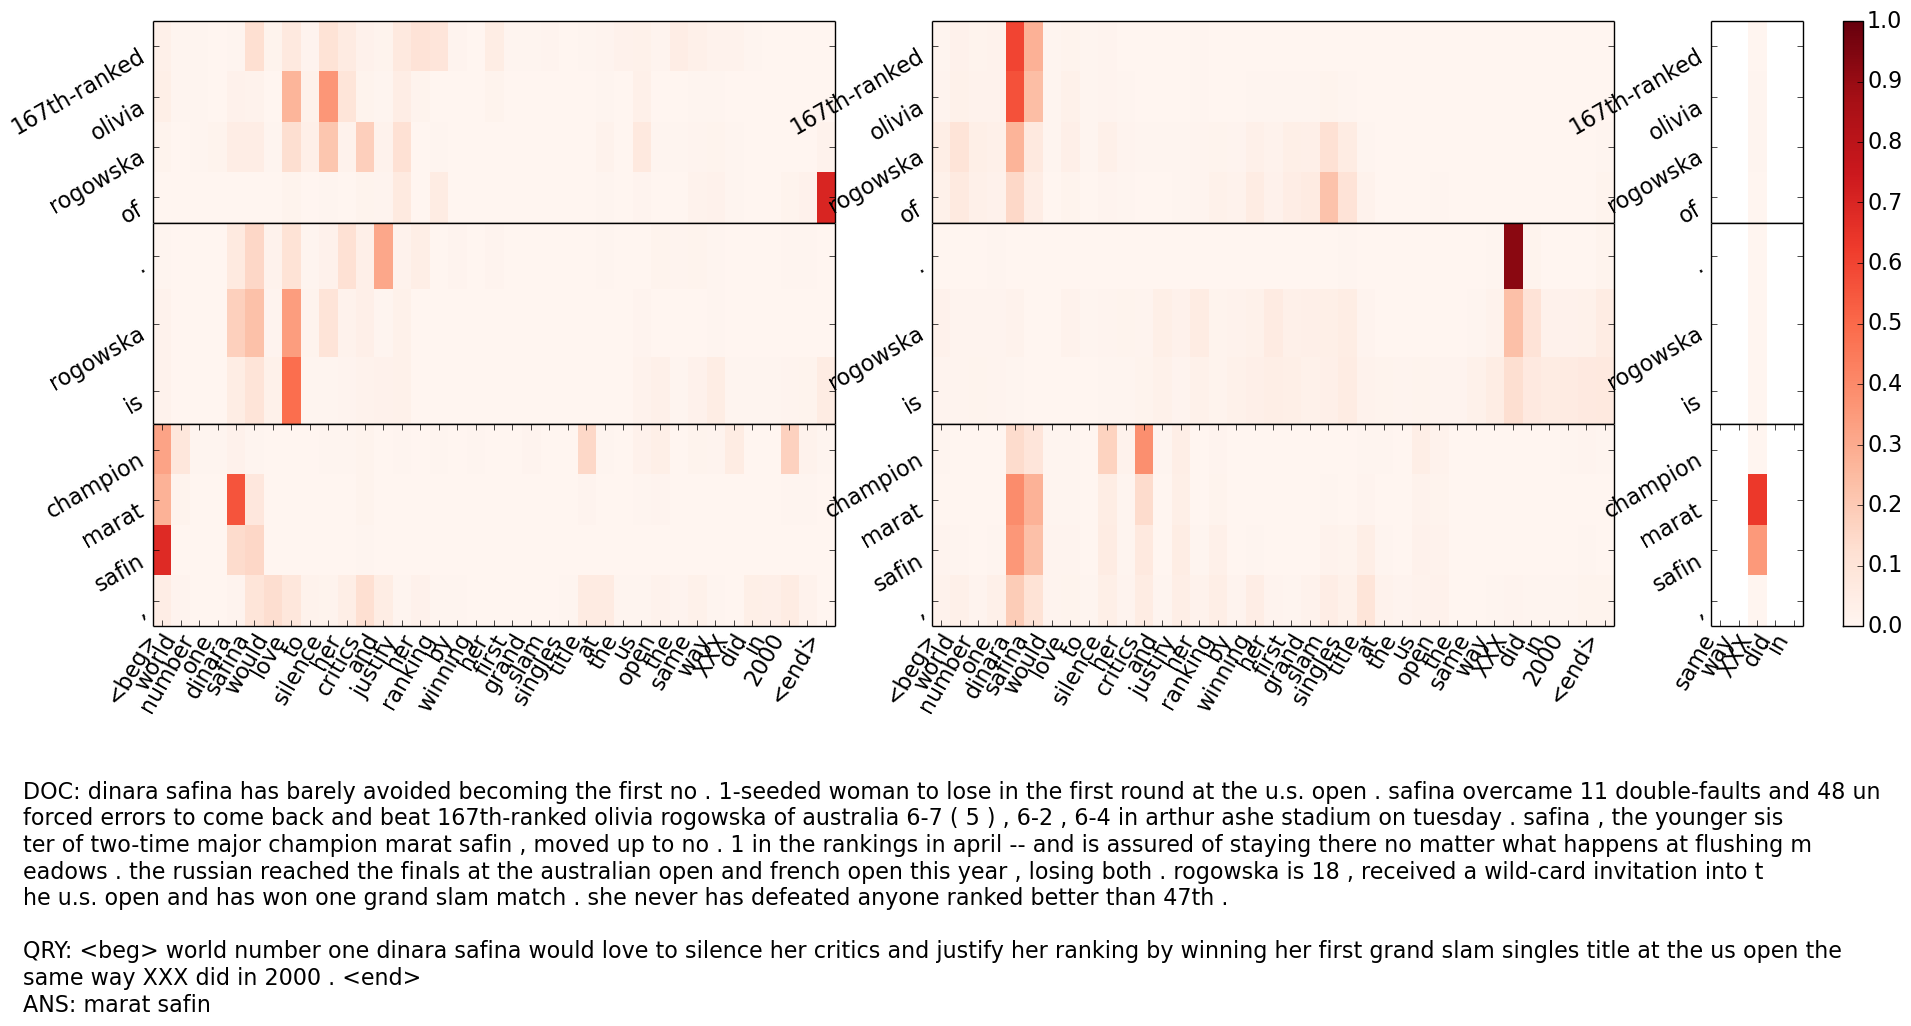
\includegraphics[width=\linewidth]{attention_plots/AFP_ENG_20090829_0124_question.png}
\end{subfigure}
\end{figure*}

\iffalse
\section{Detailed Analysis}
\label{sec:error}
\subsection{Linguistic Feature Annotation}
To gain insights about the neural readers' behavior at a more detailed level, we randomly sampled 100 questions from the test set of CNN and manually annotated their linguistic features\footnote{We plan to make the annotated questions publicly available if the manuscript is accepted for publication.}. For each question, features that may potentially correlate with the neural readers' performance were extracted, as outlined in Table \ref{tab:features}. In this paper, we primarily focus on two types of linguistic features:


\begin{table*}[t]
\centering
\resizebox{\linewidth}{!}{
  \begin{tabular}{lll}
  \toprule
  \multicolumn{3}{l}{\textbf{Plain Features}} \\ \midrule
  Feature Name          & Value          & \multicolumn{1}{c}{Description}                                                                                  \\ \midrule
  Document Length (\texttt{DL})       & $\mathbb{R}_+$   & Total number of words in the context in logarithmic scale, namely $\log(|d|)$.                                            \\
  Query Length (\texttt{QL})          & $\mathbb{N}_+$ & Total number of words in the query, namely $|q|$.                                                                 \\
  Answer Frequency (\texttt{AF})     & $\mathbb{N}_+$ & Count of correct answers in $d$.                                                                                 \\
  Answer First Location (\texttt{AFL}) & $[0,1]$          & Distance from the 1st answer occurrence to the beginning of $d$, normalized by $|d|$. \\
  Answer Last Location (\texttt{ALL}) & $[0,1]$          & Distance from the last answer occurrence to the end of $d$, normalized by $|d|$.     \\ \midrule
  \multicolumn{3}{l}{\textbf{Semantic Features}}                                                                                       \\
  \midrule
  Feature Name          & Value          & \multicolumn{1}{c}{Description}                                                                                  \\
  \midrule
  Evidence Sentence (\texttt{ES})    & $\mathbb{N}_+$     & Number of evidence sentences in $d$ needed in order to correctly answer the query.                    \\
  N-gram (\texttt{NG})              & $\{0,1\}$            & If there is an N-gram in $d$ that overlaps with the correct answer and its context in $q$.                         \\
  Paraphrase (\texttt{P})        & $\{0,1\}$            & Whether the query is rephrased in the document.                                                                  \\
  Logical Reasoning (\texttt{LR})    & $\{0,1\}$            & If multiple independent facts need to be logically combined to obtain the answer.               \\
  Temporal Reasoning (\texttt{TR})   & $\{0,1\}$            & Special case of Logical Reasoning, where the temporal order of events matters.        \\ \bottomrule                          
  \end{tabular}
}
\caption{Annotated linguistic features for the 100 CNN questions.}
\label{tab:features}
\end{table*}

\begin{itemize}
\item \emph{Plain Features} that are automatically annotated by scripts, such as document/query length, answer frequency, etc. Most of them are straightforward meta-information about the question.
\item \emph{Semantic Features} that are manually annotated by a human expert. For example, whether logical reasoning is necessary to obtain the correct answer. Features of this type are arguably more precise indicators about the intrinsic semantic nature of any given question.
\end{itemize}

\begin{figure}[t]
\centering
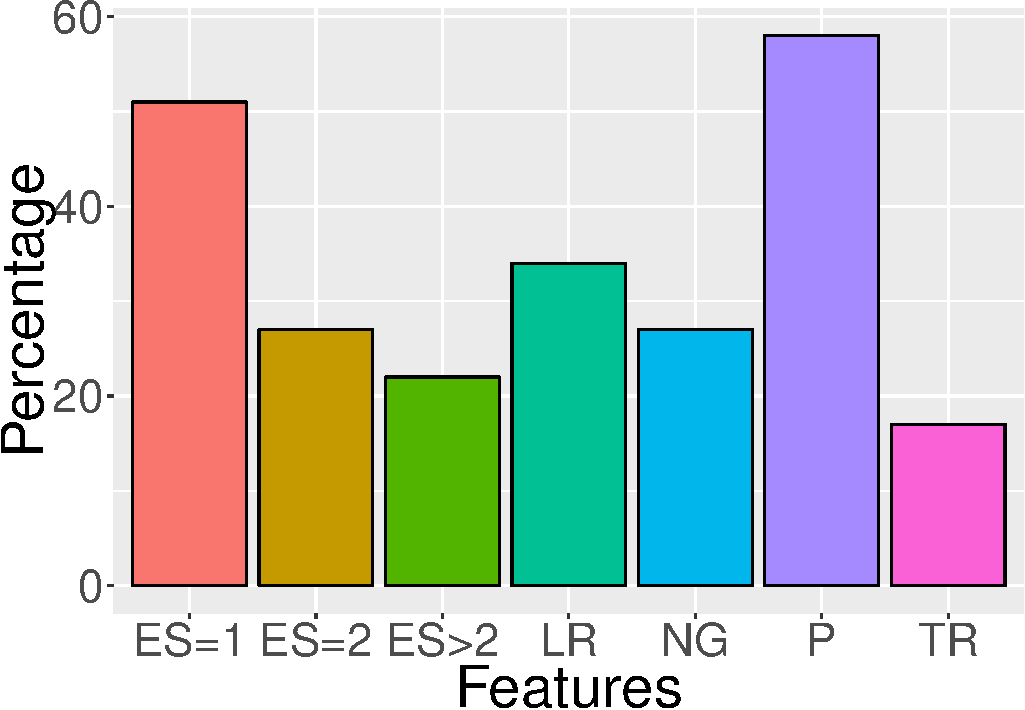
\includegraphics[width=0.7\linewidth]{semantic-feature-stats.pdf}
\caption{Corpus statistics of manually annotated semantic features.
The $y$-axis stands for the percentage of questions among the 100 samples conditioned on each feature.}
\label{fig:sf-stats}
\end{figure}

Figure \ref{fig:sf-stats} summarizes the corpus statistics regarding semantic features. Interestingly, the figure shows that the majority of the questions can be answered based on N-grams or paraphrases with less than two evidence sentences. This suggests relying on accuracy as the sole metric for model evaluation could be misleading, as a high accuracy can be achieved by pure ``memorizing'' regardless of the model's capability of capturing real semantics.

\subsection{Conditional Performance}
In this subsection, we investigate the performance of several representative models conditioned on a subset of questions with certain semantic features. As we discussed above, breaking down overall accuracy into multiple conditional performances will enable us to get a more comprehensive view about the strength and weakness of different architectures.

Four models are chosen for comparison: (1) the word distance benchmark (WD), a simple yet strong baseline relying on word distance measurements; (2) the Deep LSTM Reader, a representative LSTM-based neural architecture
\citep{hermann2015teaching}; (3) the Attention Sum (AS) Reader, which achieves the state-of-the-art performance over several text comprehension tasks \citep{kadlec2016text}; (4) GA reader, our proposed model.

Results are reported in Figure \ref{fig:cond-performance},
where the conditional performance of GA reader dominates other baselines except for temporal reasoning, showing a balanced strength in handling questions across the spectrum. While all models show weakness in reasoning with multiple facts (\texttt{ES} $\ge 3$), we notice GA reader wins with a good margin in terms of combining two facts (\texttt{ES} $=2$), suggesting its advantages in preliminary logical reasoning. The results also empirically justify the merits of attention sum, as both AS and GA readers significantly outperform WD and vanilla deep LSTM over all question types.

\begin{figure}[t]
\centering
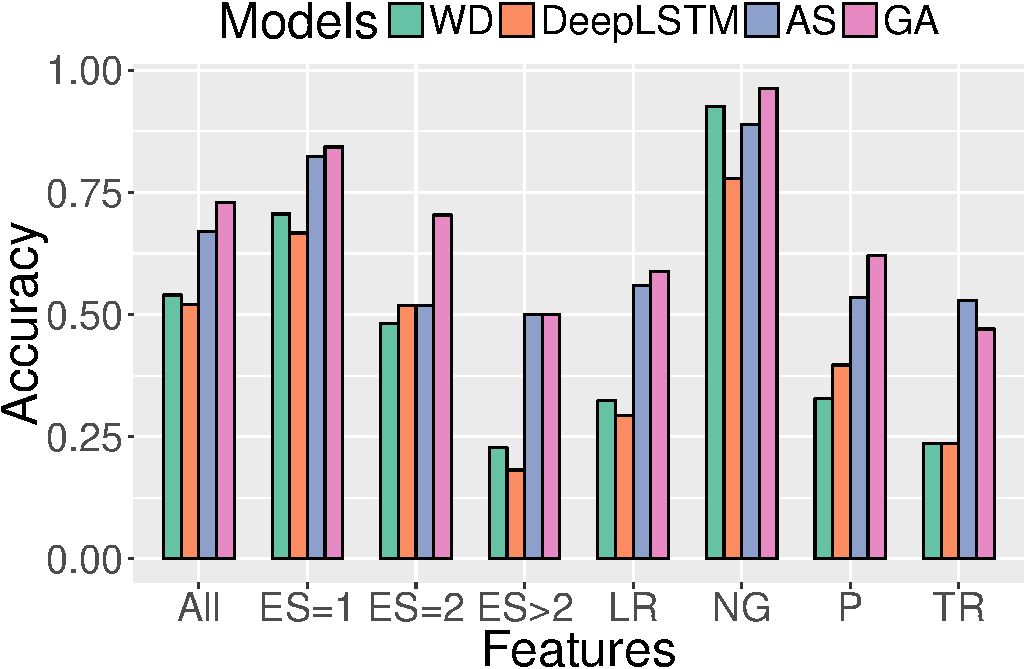
\includegraphics[width=0.9\linewidth]{cond-performance.pdf}
\caption{Conditional performance of the word distance model, Deep LSTM, AS and GA readers over the 100 CNN questions with respect to different semantic features. ``All'' refers to the overall performance on the 100 questions without conditions.}
\label{fig:cond-performance}
\end{figure}

\subsection{Sensitivity Analysis}
With the linguistic features in Table \ref{tab:features}, each of the 100 CNN sample questions can be summarized as an 11-dimensional vector $x$ (10 features plus an intercept). Let $y = 1$ if the question has been correctly answered and $y=0$ otherwise. One can therefore quantitatively characterize the sensitivity of the neural readers' performance w.r.t.\ different linguistic features by fitting a linear regression model where $x$ and $y$ are treated as explanatory and response variables, respectively
\footnote{Before regression, all features were normalized to the range of $[0,1]$ to make their scales comparable.}.
The resulting regression coefficients and $p$-values can effectively summarize which features are influential to the model performance.

\begin{figure}[t]
\centering
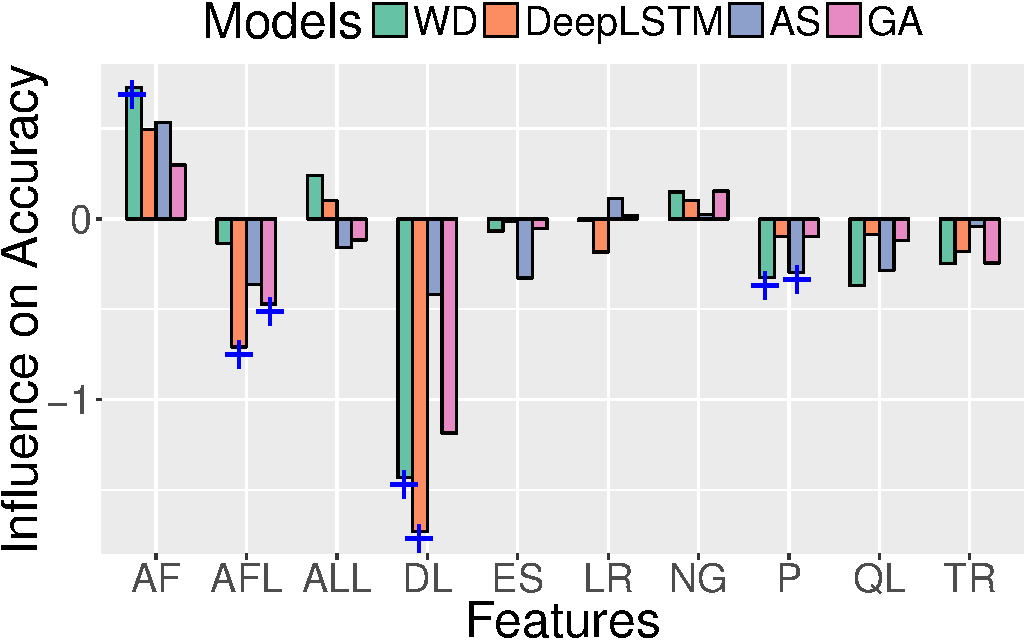
\includegraphics[width=0.9\linewidth]{regression.pdf}
\caption{Regression coefficients of various linguistic features with respect to the performance of different models. A positive coefficient indicates a positive influence on the corresponding model's test-set accuracy and vice versa. Coefficients that are statistically significant $(\alpha= 5\%)$ are marked with ``$+$''.}
\label{fig:regression}
\end{figure}

Figure \ref{fig:regression} shows the regression coefficients associated with different linguistic features in Table \ref{tab:features}.
Besides the known effect of DL and AF that have been discussed in the literature, we see the involvement of logical reasoning (LR), paraphrases (P) and multiple evidence sentences (ES) consistently lead to decreased performance for all models,
though multi-layered architectures (DeepLSTM, GA) are empirically more robust than single-layer (AS) or shallow (WD) ones in those aspects. 
Interestingly, Figure \ref{fig:regression} also shows AFL is playing a crucial role.
One possible explanation is that questions whose answers appear early tend to be relatively easier in nature.
Meanwhile,
it is not hard to verify that with high probability AFL will be negatively correlated with AF, a quantity known to have significance influence on the performance of most models.
\fi


\end{document}
